
%% bare_jrnl.tex
%% V1.3
%% 2007/01/11
%% by Michael Shell
%% see http://www.michaelshell.org/
%% for current contact information.
%%
%% This is a skeleton file demonstrating the use of IEEEtran.cls
%% (requires IEEEtran.cls version 1.7 or later) with an IEEE journal paper.
%%
%% Support sites:
%% http://www.michaelshell.org/tex/ieeetran/
%% http://www.ctan.org/tex-archive/macros/latex/contrib/IEEEtran/
%% and
%% http://www.ieee.org/



% *** Authors should verify (and, if needed, correct) their LaTeX system  ***
% *** with the testflow diagnostic prior to trusting their LaTeX platform ***
% *** with production work. IEEE's font choices can trigger bugs that do  ***
% *** not appear when using other class files.                            ***
% The testflow support page is at:
% http://www.michaelshell.org/tex/testflow/


%%*************************************************************************
%% Legal Notice:
%% This code is offered as-is without any warranty either expressed or
%% implied; without even the implied warranty of MERCHANTABILITY or
%% FITNESS FOR A PARTICULAR PURPOSE! 
%% User assumes all risk.
%% In no event shall IEEE or any contributor to this code be liable for
%% any damages or losses, including, but not limited to, incidental,
%% consequential, or any other damages, resulting from the use or misuse
%% of any information contained here.
%%
%% All comments are the opinions of their respective authors and are not
%% necessarily endorsed by the IEEE.
%%
%% This work is distributed under the LaTeX Project Public License (LPPL)
%% ( http://www.latex-project.org/ ) version 1.3, and may be freely used,
%% distributed and modified. A copy of the LPPL, version 1.3, is included
%% in the base LaTeX documentation of all distributions of LaTeX released
%% 2003/12/01 or later.
%% Retain all contribution notices and credits.
%% ** Modified files should be clearly indicated as such, including  **
%% ** renaming them and changing author support contact information. **
%%
%% File list of work: IEEEtran.cls, IEEEtran_HOWTO.pdf, bare_adv.tex,
%%                    bare_conf.tex, bare_jrnl.tex, bare_jrnl_compsoc.tex
%%*************************************************************************

% Note that the a4paper option is mainly intended so that authors in
% countries using A4 can easily print to A4 and see how their papers will
% look in print - the typesetting of the document will not typically be
% affected with changes in paper size (but the bottom and side margins will).
% Use the testflow package mentioned above to verify correct handling of
% both paper sizes by the user's LaTeX system.
%
% Also note that the "draftcls" or "draftclsnofoot", not "draft", option
% should be used if it is desired that the figures are to be displayed in
% draft mode.
%
\documentclass[journal]{IEEEtran}
%
% If IEEEtran.cls has not been installed into the LaTeX system files,
% manually specify the path to it like:
% \documentclass[journal]{../sty/IEEEtran}





% Some very useful LaTeX packages include:
% (uncomment the ones you want to load)


% *** MISC UTILITY PACKAGES ***
%
%\usepackage{ifpdf}
% Heiko Oberdiek's ifpdf.sty is very useful if you need conditional
% compilation based on whether the output is pdf or dvi.
% usage:
% \ifpdf
%   % pdf code
% \else
%   % dvi code
% \fi
% The latest version of ifpdf.sty can be obtained from:
% http://www.ctan.org/tex-archive/macros/latex/contrib/oberdiek/
% Also, note that IEEEtran.cls V1.7 and later provides a builtin
% \ifCLASSINFOpdf conditional that works the same way.
% When switching from latex to pdflatex and vice-versa, the compiler may
% have to be run twice to clear warning/error messages.






% *** CITATION PACKAGES ***
%
%\usepackage{cite}
% cite.sty was written by Donald Arseneau
% V1.6 and later of IEEEtran pre-defines the format of the cite.sty package
% \cite{} output to follow that of IEEE. Loading the cite package will
% result in citation numbers being automatically sorted and properly
% "compressed/ranged". e.g., [1], [9], [2], [7], [5], [6] without using
% cite.sty will become [1], [2], [5]--[7], [9] using cite.sty. cite.sty's
% \cite will automatically add leading space, if needed. Use cite.sty's
% noadjust option (cite.sty V3.8 and later) if you want to turn this off.
% cite.sty is already installed on most LaTeX systems. Be sure and use
% version 4.0 (2003-05-27) and later if using hyperref.sty. cite.sty does
% not currently provide for hyperlinked citations.
% The latest version can be obtained at:
% http://www.ctan.org/tex-archive/macros/latex/contrib/cite/
% The documentation is contained in the cite.sty file itself.






% *** GRAPHICS RELATED PACKAGES ***
%
\usepackage{graphicx}
\graphicspath{{./figures/}}
\DeclareGraphicsExtensions{.png}

\ifCLASSINFOpdf
  % \usepackage[pdftex]{graphicx}
  % declare the path(s) where your graphic files are
  % \graphicspath{{../pdf/}{../jpeg/}}
  % and their extensions so you won't have to specify these with
  % every instance of \includegraphics
  % \DeclareGraphicsExtensions{.pdf,.jpeg,.png}
\else
  % or other class option (dvipsone, dvipdf, if not using dvips). graphicx
  % will default to the driver specified in the system graphics.cfg if no
  % driver is specified.
  % \usepackage[dvips]{graphicx}
  % declare the path(s) where your graphic files are
  % \graphicspath{{../eps/}}
  % and their extensions so you won't have to specify these with
  % every instance of \includegraphics
  % \DeclareGraphicsExtensions{.eps}
\fi
% graphicx was written by David Carlisle and Sebastian Rahtz. It is
% required if you want graphics, photos, etc. graphicx.sty is already
% installed on most LaTeX systems. The latest version and documentation can
% be obtained at: 
% http://www.ctan.org/tex-archive/macros/latex/required/graphics/
% Another good source of documentation is "Using Imported Graphics in
% LaTeX2e" by Keith Reckdahl which can be found as epslatex.ps or
% epslatex.pdf at: http://www.ctan.org/tex-archive/info/
%
% latex, and pdflatex in dvi mode, support graphics in encapsulated
% postscript (.eps) format. pdflatex in pdf mode supports graphics
% in .pdf, .jpeg, .png and .mps (metapost) formats. Users should ensure
% that all non-photo figures use a vector format (.eps, .pdf, .mps) and
% not a bitmapped formats (.jpeg, .png). IEEE frowns on bitmapped formats
% which can result in "jaggedy"/blurry rendering of lines and letters as
% well as large increases in file sizes.
%
% You can find documentation about the pdfTeX application at:
% http://www.tug.org/applications/pdftex





% *** MATH PACKAGES ***
%
%\usepackage[cmex10]{amsmath}
% A popular package from the American Mathematical Society that provides
% many useful and powerful commands for dealing with mathematics. If using
% it, be sure to load this package with the cmex10 option to ensure that
% only type 1 fonts will utilized at all point sizes. Without this option,
% it is possible that some math symbols, particularly those within
% footnotes, will be rendered in bitmap form which will result in a
% document that can not be IEEE Xplore compliant!
%
% Also, note that the amsmath package sets \interdisplaylinepenalty to 10000
% thus preventing page breaks from occurring within multiline equations. Use:
%\interdisplaylinepenalty=2500
% after loading amsmath to restore such page breaks as IEEEtran.cls normally
% does. amsmath.sty is already installed on most LaTeX systems. The latest
% version and documentation can be obtained at:
% http://www.ctan.org/tex-archive/macros/latex/required/amslatex/math/





% *** SPECIALIZED LIST PACKAGES ***
%
%\usepackage{algorithmic}
% algorithmic.sty was written by Peter Williams and Rogerio Brito.
% This package provides an algorithmic environment fo describing algorithms.
% You can use the algorithmic environment in-text or within a figure
% environment to provide for a floating algorithm. Do NOT use the algorithm
% floating environment provided by algorithm.sty (by the same authors) or
% algorithm2e.sty (by Christophe Fiorio) as IEEE does not use dedicated
% algorithm float types and packages that provide these will not provide
% correct IEEE style captions. The latest version and documentation of
% algorithmic.sty can be obtained at:
% http://www.ctan.org/tex-archive/macros/latex/contrib/algorithms/
% There is also a support site at:
% http://algorithms.berlios.de/index.html
% Also of interest may be the (relatively newer and more customizable)
% algorithmicx.sty package by Szasz Janos:
% http://www.ctan.org/tex-archive/macros/latex/contrib/algorithmicx/




% *** ALIGNMENT PACKAGES ***
%
%\usepackage{array}
% Frank Mittelbach's and David Carlisle's array.sty patches and improves
% the standard LaTeX2e array and tabular environments to provide better
% appearance and additional user controls. As the default LaTeX2e table
% generation code is lacking to the point of almost being broken with
% respect to the quality of the end results, all users are strongly
% advised to use an enhanced (at the very least that provided by array.sty)
% set of table tools. array.sty is already installed on most systems. The
% latest version and documentation can be obtained at:
% http://www.ctan.org/tex-archive/macros/latex/required/tools/


%\usepackage{mdwmath}
%\usepackage{mdwtab}
% Also highly recommended is Mark Wooding's extremely powerful MDW tools,
% especially mdwmath.sty and mdwtab.sty which are used to format equations
% and tables, respectively. The MDWtools set is already installed on most
% LaTeX systems. The lastest version and documentation is available at:
% http://www.ctan.org/tex-archive/macros/latex/contrib/mdwtools/


% IEEEtran contains the IEEEeqnarray family of commands that can be used to
% generate multiline equations as well as matrices, tables, etc., of high
% quality.


%\usepackage{eqparbox}
% Also of notable interest is Scott Pakin's eqparbox package for creating
% (automatically sized) equal width boxes - aka "natural width parboxes".
% Available at:
% http://www.ctan.org/tex-archive/macros/latex/contrib/eqparbox/





% *** SUBFIGURE PACKAGES ***
%\usepackage[tight,footnotesize]{subfigure}
% subfigure.sty was written by Steven Douglas Cochran. This package makes it
% easy to put subfigures in your figures. e.g., "Figure 1a and 1b". For IEEE
% work, it is a good idea to load it with the tight package option to reduce
% the amount of white space around the subfigures. subfigure.sty is already
% installed on most LaTeX systems. The latest version and documentation can
% be obtained at:
% http://www.ctan.org/tex-archive/obsolete/macros/latex/contrib/subfigure/
% subfigure.sty has been superceeded by subfig.sty.



%\usepackage[caption=false]{caption}
%\usepackage[font=footnotesize]{subfig}
% subfig.sty, also written by Steven Douglas Cochran, is the modern
% replacement for subfigure.sty. However, subfig.sty requires and
% automatically loads Axel Sommerfeldt's caption.sty which will override
% IEEEtran.cls handling of captions and this will result in nonIEEE style
% figure/table captions. To prevent this problem, be sure and preload
% caption.sty with its "caption=false" package option. This is will preserve
% IEEEtran.cls handing of captions. Version 1.3 (2005/06/28) and later 
% (recommended due to many improvements over 1.2) of subfig.sty supports
% the caption=false option directly:
%\usepackage[caption=false,font=footnotesize]{subfig}
%
% The latest version and documentation can be obtained at:
% http://www.ctan.org/tex-archive/macros/latex/contrib/subfig/
% The latest version and documentation of caption.sty can be obtained at:
% http://www.ctan.org/tex-archive/macros/latex/contrib/caption/




% *** FLOAT PACKAGES ***
%
%\usepackage{fixltx2e}
% fixltx2e, the successor to the earlier fix2col.sty, was written by
% Frank Mittelbach and David Carlisle. This package corrects a few problems
% in the LaTeX2e kernel, the most notable of which is that in current
% LaTeX2e releases, the ordering of single and double column floats is not
% guaranteed to be preserved. Thus, an unpatched LaTeX2e can allow a
% single column figure to be placed prior to an earlier double column
% figure. The latest version and documentation can be found at:
% http://www.ctan.org/tex-archive/macros/latex/base/



%\usepackage{stfloats}
% stfloats.sty was written by Sigitas Tolusis. This package gives LaTeX2e
% the ability to do double column floats at the bottom of the page as well
% as the top. (e.g., "\begin{figure*}[!b]" is not normally possible in
% LaTeX2e). It also provides a command:
%\fnbelowfloat
% to enable the placement of footnotes below bottom floats (the standard
% LaTeX2e kernel puts them above bottom floats). This is an invasive package
% which rewrites many portions of the LaTeX2e float routines. It may not work
% with other packages that modify the LaTeX2e float routines. The latest
% version and documentation can be obtained at:
% http://www.ctan.org/tex-archive/macros/latex/contrib/sttools/
% Documentation is contained in the stfloats.sty comments as well as in the
% presfull.pdf file. Do not use the stfloats baselinefloat ability as IEEE
% does not allow \baselineskip to stretch. Authors submitting work to the
% IEEE should note that IEEE rarely uses double column equations and
% that authors should try to avoid such use. Do not be tempted to use the
% cuted.sty or midfloat.sty packages (also by Sigitas Tolusis) as IEEE does
% not format its papers in such ways.


%\ifCLASSOPTIONcaptionsoff
%  \usepackage[nomarkers]{endfloat}
% \let\MYoriglatexcaption\caption
% \renewcommand{\caption}[2][\relax]{\MYoriglatexcaption[#2]{#2}}
%\fi
% endfloat.sty was written by James Darrell McCauley and Jeff Goldberg.
% This package may be useful when used in conjunction with IEEEtran.cls'
% captionsoff option. Some IEEE journals/societies require that submissions
% have lists of figures/tables at the end of the paper and that
% figures/tables without any captions are placed on a page by themselves at
% the end of the document. If needed, the draftcls IEEEtran class option or
% \CLASSINPUTbaselinestretch interface can be used to increase the line
% spacing as well. Be sure and use the nomarkers option of endfloat to
% prevent endfloat from "marking" where the figures would have been placed
% in the text. The two hack lines of code above are a slight modification of
% that suggested by in the endfloat docs (section 8.3.1) to ensure that
% the full captions always appear in the list of figures/tables - even if
% the user used the short optional argument of \caption[]{}.
% IEEE papers do not typically make use of \caption[]'s optional argument,
% so this should not be an issue. A similar trick can be used to disable
% captions of packages such as subfig.sty that lack options to turn off
% the subcaptions:
% For subfig.sty:
% \let\MYorigsubfloat\subfloat
% \renewcommand{\subfloat}[2][\relax]{\MYorigsubfloat[]{#2}}
% For subfigure.sty:
% \let\MYorigsubfigure\subfigure
% \renewcommand{\subfigure}[2][\relax]{\MYorigsubfigure[]{#2}}
% However, the above trick will not work if both optional arguments of
% the \subfloat/subfig command are used. Furthermore, there needs to be a
% description of each subfigure *somewhere* and endfloat does not add
% subfigure captions to its list of figures. Thus, the best approach is to
% avoid the use of subfigure captions (many IEEE journals avoid them anyway)
% and instead reference/explain all the subfigures within the main caption.
% The latest version of endfloat.sty and its documentation can obtained at:
% http://www.ctan.org/tex-archive/macros/latex/contrib/endfloat/
%
% The IEEEtran \ifCLASSOPTIONcaptionsoff conditional can also be used
% later in the document, say, to conditionally put the References on a 
% page by themselves.





% *** PDF, URL AND HYPERLINK PACKAGES ***
%
%\usepackage{url}
% url.sty was written by Donald Arseneau. It provides better support for
% handling and breaking URLs. url.sty is already installed on most LaTeX
% systems. The latest version can be obtained at:
% http://www.ctan.org/tex-archive/macros/latex/contrib/misc/
% Read the url.sty source comments for usage information. Basically,
% \url{my_url_here}.





% *** Do not adjust lengths that control margins, column widths, etc. ***
% *** Do not use packages that alter fonts (such as pslatex).         ***
% There should be no need to do such things with IEEEtran.cls V1.6 and later.
% (Unless specifically asked to do so by the journal or conference you plan
% to submit to, of course. )


% correct bad hyphenation here
\hyphenation{op-tical net-works semi-conduc-tor}


\begin{document}
%
% paper title
% can use linebreaks \\ within to get better formatting as desired
\title{Elevavator Controller}
%
%
% author names and IEEE memberships
% note positions of commas and nonbreaking spaces ( ~ ) LaTeX will not break
% a structure at a ~ so this keeps an author's name from being broken across
% two lines.
% use \thanks{} to gain access to the first footnote area
% a separate \thanks must be used for each paragraph as LaTeX2e's \thanks
% was not built to handle multiple paragraphs
%

\author{Taixing~Bi, Wesley~Eledui, Justin~Gay, and~John~Wilkes}% <-this % stops a space

% note the % following the last \IEEEmembership and also \thanks - 
% these prevent an unwanted space from occurring between the last author name
% and the end of the author line. i.e., if you had this:
% 
% \author{....lastname \thanks{...} \thanks{...} }
%                     ^------------^------------^----Do not want these spaces!
%
% a space would be appended to the last name and could cause every name on that
% line to be shifted left slightly. This is one of those "LaTeX things". For
% instance, "\textbf{A} \textbf{B}" will typeset as "A B" not "AB". To get
% "AB" then you have to do: "\textbf{A}\textbf{B}"
% \thanks is no different in this regard, so shield the last } of each \thanks
% that ends a line with a % and do not let a space in before the next \thanks.
% Spaces after \IEEEmembership other than the last one are OK (and needed) as
% you are supposed to have spaces between the names. For what it is worth,
% this is a minor point as most people would not even notice if the said evil
% space somehow managed to creep in.



% The paper headers
%\markboth{Journal of \LaTeX\ Class Files,~Vol.~6, No.~1, January~2007}%
%{Shell \MakeLowercase{\textit{et al.}}: Bare Demo of IEEEtran.cls for Journals}
% The only time the second header will appear is for the odd numbered pages
% after the title page when using the twoside option.
% 
% *** Note that you probably will NOT want to include the author's ***
% *** name in the headers of peer review papers.                   ***
% You can use \ifCLASSOPTIONpeerreview for conditional compilation here if
% you desire.




% If you want to put a publisher's ID mark on the page you can do it like
% this:
%\IEEEpubid{0000--0000/00\$00.00~\copyright~2007 IEEE}
% Remember, if you use this you must call \IEEEpubidadjcol in the second
% column for its text to clear the IEEEpubid mark.



% use for special paper notices
%\IEEEspecialpapernotice{(Invited Paper)}




% make the title area
\maketitle


%\begin{abstract}
%\boldmath
%The abstract goes here.
%\end{abstract}
% IEEEtran.cls defaults to using nonbold math in the Abstract.
% This preserves the distinction between vectors and scalars. However,
% if the journal you are submitting to favors bold math in the abstract,
% then you can use LaTeX's standard command \boldmath at the very start
% of the abstract to achieve this. Many IEEE journals frown on math
% in the abstract anyway.

% Note that keywords are not normally used for peerreview papers.
\begin{IEEEkeywords}
elevator, controller.
\end{IEEEkeywords}






% For peer review papers, you can put extra information on the cover
% page as needed:
% \ifCLASSOPTIONpeerreview
% \begin{center} \bfseries EDICS Category: 3-BBND \end{center}
% \fi
%
% For peerreview papers, this IEEEtran command inserts a page break and
% creates the second title. It will be ignored for other modes.
\IEEEpeerreviewmaketitle



\section{Design Description}
% The very first letter is a 2 line initial drop letter followed
% by the rest of the first word in caps.
% 
% form to use if the first word consists of a single letter:
% \IEEEPARstart{A}{demo} file is ....
% 
% form to use if you need the single drop letter followed by
% normal text (unknown if ever used by IEEE):
% \IEEEPARstart{A}{}demo file is ....
% 
% Some journals put the first two words in caps:
% \IEEEPARstart{T}{his demo} file is ....
% 
% Here we have the typical use of a "T" for an initial drop letter
% and "HIS" in caps to complete the first word.
% You must have at least 2 lines in the paragraph with the drop letter
% (should never be an issue)
\IEEEPARstart{T}{his} model is a controller for an elevator that services three floors. It has nine inputs and two outputs. There are four external buttons: one on the first floor to request to go up, two on the second floor to request to go up and down, and one on the third floor to request to go down. There are also three buttons internal to the elevator to request to go to each floor. The elevator uses two sensors. The first is a door sensor. This is used to ensure that the elevator doors have closed before moving to another floor. The input is 0 when the doors are open and 1 when the doors have closed. The second sensor is a floor sensor. This input informs the controller when the elevator has arrived at a new floor. It is a two-bit value that indicates the floor the elevator is currently on (01$_{2}$ – floor 1, 10$_{2}$ – floor 2, 11$_{2}$ – floor 3). The two outputs of the elevator controller are door controller and elevator direction signals. The door controller sets whether the door is open or closed. When it is 0, the doors open, and when it is 1, the doors close. The elevator direction output is a two-bit value that controls the direction in which the elevator is traveling. A value of 00$_{2}$ keeps the elevator stationary, 01$_{2}$ moves the elevator up, and 10$_{2}$ moves the elevator down.

%\hfill mds
 
%\hfill January 11, 2007

%\subsection{Subsection Heading Here}
%Subsection text here.

% needed in second column of first page if using \IEEEpubid
%\IEEEpubidadjcol

%\subsubsection{Subsubsection Heading Here}
%Subsubsection text here.


% An example of a floating figure using the graphicx package.
% Note that \label must occur AFTER (or within) \caption.
% For figures, \caption should occur after the \includegraphics.
% Note that IEEEtran v1.7 and later has special internal code that
% is designed to preserve the operation of \label within \caption
% even when the captionsoff option is in effect. However, because
% of issues like this, it may be the safest practice to put all your
% \label just after \caption rather than within \caption{}.
%
% Reminder: the "draftcls" or "draftclsnofoot", not "draft", class
% option should be used if it is desired that the figures are to be
% displayed while in draft mode.
%
%\begin{figure}[!t]
%\centering
%\includegraphics[width=2.5in]{myfigure}
% where an .eps filename suffix will be assumed under latex, 
% and a .pdf suffix will be assumed for pdflatex; or what has been declared
% via \DeclareGraphicsExtensions.
%\caption{Simulation Results}
%\label{fig_sim}
%\end{figure}

% Note that IEEE typically puts floats only at the top, even when this
% results in a large percentage of a column being occupied by floats.


% An example of a double column floating figure using two subfigures.
% (The subfig.sty package must be loaded for this to work.)
% The subfigure \label commands are set within each subfloat command, the
% \label for the overall figure must come after \caption.
% \hfil must be used as a separator to get equal spacing.
% The subfigure.sty package works much the same way, except \subfigure is
% used instead of \subfloat.
%
%\begin{figure*}[!t]
%\centerline{\subfloat[Case I]\includegraphics[width=2.5in]{subfigcase1}%
%\label{fig_first_case}}
%\hfil
%\subfloat[Case II]{\includegraphics[width=2.5in]{subfigcase2}%
%\label{fig_second_case}}}
%\caption{Simulation results}
%\label{fig_sim}
%\end{figure*}
%
% Note that often IEEE papers with subfigures do not employ subfigure
% captions (using the optional argument to \subfloat), but instead will
% reference/describe all of them (a), (b), etc., within the main caption.


% An example of a floating table. Note that, for IEEE style tables, the 
% \caption command should come BEFORE the table. Table text will default to
% \footnotesize as IEEE normally uses this smaller font for tables.
% The \label must come after \caption as always.
%
%\begin{table}[!t]
%% increase table row spacing, adjust to taste
%\renewcommand{\arraystretch}{1.3}
% if using array.sty, it might be a good idea to tweak the value of
% \extrarowheight as needed to properly center the text within the cells
%\caption{An Example of a Table}
%\label{table_example}
%\centering
%% Some packages, such as MDW tools, offer better commands for making tables
%% than the plain LaTeX2e tabular which is used here.
%\begin{tabular}{|c||c|}
%\hline
%One & Two\\
%\hline
%Three & Four\\
%\hline
%\end{tabular}
%\end{table}


% Note that IEEE does not put floats in the very first column - or typically
% anywhere on the first page for that matter. Also, in-text middle ("here")
% positioning is not used. Most IEEE journals use top floats exclusively.
% Note that, LaTeX2e, unlike IEEE journals, places footnotes above bottom
% floats. This can be corrected via the \fnbelowfloat command of the
% stfloats package.


% State Diagram Figure
\begin{figure*}[t]
\centering
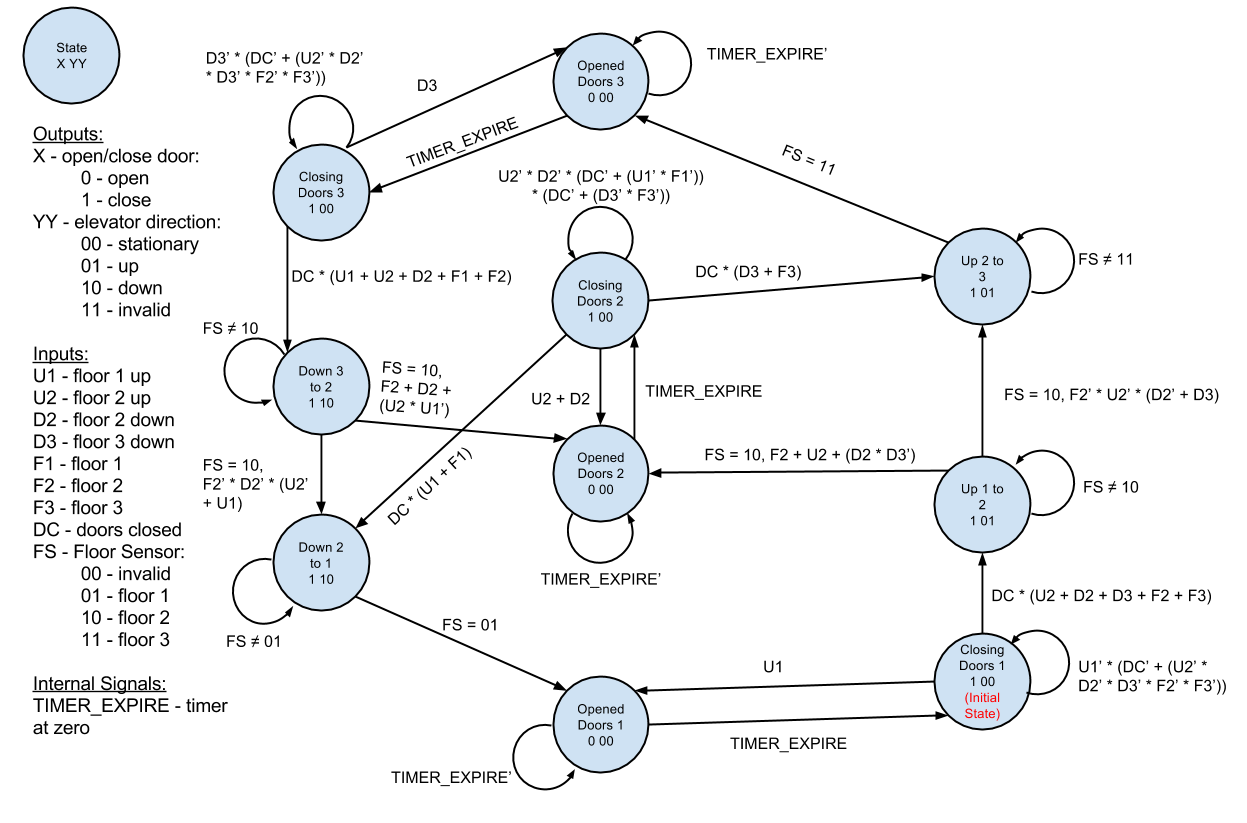
\includegraphics[width=0.9\linewidth]{ElevatorStateMachine}
\caption{State Diagram}
\label{fig_state_machine}
\end{figure*}

\section{Implementation Approach}
The elevator controller is composed of two architectures. The main architecture is the state machine. 
The second is the door timer.

\subsection{State Machine Implementation}
The elevator controller’s main architecture is a Moore state machine with ten states. There are two states per floor: an open door state and a closed door state. There are also four states for transitioning between floors: one to go up from floor 1 to floor 2, one to go up from floor 2 to floor 3, one to go down from floor 3 to floor 2, and one to go down from floor 2 to floor 1. When in the closed door state of any floor, the elevator will stay stationary while there are no button presses. If a request button is pressed on the floor that the elevator is on, the elevator will transition to the open doors state. As soon as the elevator enters this state, it starts a timer. When this timer expires, the elevator will enter the closed doors state. If an external button is pressed on a different floor than that which the elevator is on, or an internal button is pressed to request to go to a different floor, the elevator will exit the closed doors state and enter a state to travel either up or down depending upon the request. Also, note that to exit the doors closed state, the input from the door sensor must be high indicating that the door has finished closing.

\subsection{Door Timer}
There is also a timer architecture used in the elevator controller. This timer specifies how long the controller stays in the open door state. The reason for having this timer is twofold. First, when the elevator reaches a floor and all passengers get off, most elevators close their doors and stay at the current floor until there is a request on another floor. The timer ensures that the elevator does not stay on a floor with the doors open for extended periods of time. The second, and most important, reason for the timer is to ensure that passengers have enough time to exit the elevator. Before the timer was added, the elevator would enter the closed door state whenever there was a button request. However, this caused problems in certain situations. For example, assume a button was pressed on the third floor when the elevator arrived at the first or second floor. In this case, the elevator would begin to open its doors but then sense the third floor request. It would then immediately close its doors again before the passengers could exit. Having the timer keeps the doors open for a specified time giving passengers a chance to enter and exit the elevator.

\subsection{Button Input Latching}
Internal variables are used in the state machine architecture to store which buttons have been pressed. This prevents a passenger from having to continuously hold down a button to request the elevator. Instead, when a passenger presses a button, the button press is latched in and not cleared until the request is serviced. For example, if a passenger on the first floor enters the elevator and presses the third floor button, the request to go to the third floor will be latched, thus preventing him from having to hold down the button until he arrives at the third floor. When the third floor is reached, the request is cleared.

\subsection{Second Floor Special Cases}
The state machine has to handle certain special cases when servicing the second floor. This is because the elevator can travel up or down from this floor. When traveling past the second floor, the elevator will stop to pick up passengers who are traveling in the same direction. For example, if the elevator is carrying a passenger down from the third floor to the first, it will stop to pick up a passenger on the second floor who has pressed the down button. However, the elevator will not immediately service a request on the second floor that is opposite the direction in which it is traveling. For example, if the elevator is carrying a passenger from the third to the first floor, it will not pick up a passenger on the second floor who has pressed the up button. Instead, it will travel to the first floor and then come back up to the second floor.

The elevator controller also keeps up with the last floor it has visited. This prevents a case where the elevator could ignore requests on one floor because of continuous requests on the other two. For example, if there are passengers continuously pushing the up button on the first floor and the down button on the second floor, the elevator could repeatedly go up and down between these floors and not service requests on the third floor. By keeping track of the last floor visited, the controller can ensure it will service a request on a floor it has not visited in a while over a request on the floor from which it just came. Keeping track of the last floor visited also prevents the case where a malicious user on the second floor could disrupt the direction of travel. In this case, the elevator is carrying a passenger from the first floor to the third and stops on the second floor because a passenger there has pushed the up button. However, when this passenger gets on, he presses the first floor button even though he previously requested to go up. Without knowing what floor it had previously visited, the elevator might go down to the first floor forcing the original passenger to have to wait to travel to the third floor. However, by remembering the last floor visited, the elevator can continue to go to the third floor forcing the malicious user to wait.


\section{Verification}
Verification of the elevator controller was accomplished with directed testing and random testing. We used two types of testing methods due to the number of different combinations that are possible with the inputs to the elevator controller.

\subsection{Directed Testing}

The idea behind directed testing was to identify specific test cases that would verify high level functionality for the elevator controller.

\subsubsection{Implementation}
A test bench was created in VHDL that read inputs to the elevator controller from a text file. The test bench consisted of two parts. The design under test (DUT) and a door sensor model (DSM). The DSM was used to provide the doors closed (DC) input to the elevator controller. The purpose of using the DSM to provide the DC input to the elevator controller was to mimic the real-world operation of a elevator controller. The DSM was triggered to start via the door output of the elevator controller. When the door output of the elevator controller goes high the DSM starts and after a few clock cycles the DSM asserts DC.

\subsubsection{Directed Test Cases}
Each directed test case was seperated by asserting reset so at the beginning of each test case the elevator was in the Closing Doors 1 state with DC high.

The first test case has a request at floor 2 to go up. When the elevator arrives at floor 2, a passenger requests internally to go to floor 3. For this test case, we expect the elevator to travel to floor 2, take on a passenger and continue to floor 3 to off-load the passenger.

The second test case has a request at floor 2 and floor 3 to go up. When the elevator arrives at floor 3, a passenger requests internally to go to floor 1. When the elevator arrives at floor 2, a passenger requests internally to go to floor 3. The elevator should travel up to floor 3 before stopping on floor 2 because the request on floor 2 is to go down. At floor 2, since the internal request is to go up to floor 3 while there is another pending request to go to floor 1, we expect the elevator to travel to floor 1 and off-load the passenger prior to handling the request at floor 2 to go to floor 3. 

The third test case has a request at floor 2 to go up. When the elevator arrives at floor 2, a passenger requests to travel to floor 1. The elevator should travel to floor 2, take on the passenger and travel back down to floor 1.

The forth test case has a request at floor 2 to go up and floor 3 to go down. When the elevator arrives at floor 2, a passenger requests to travel to floor 1. When the elevator arrives at floor 3, no passengers get on the elevator. For this test case, the elevator should travel up to floor 2, take on a passenger and then continue on to floor 3. At floor 3, since there are not passengers the elevator should leave the doors opened until the door time expires and then wait for the DC sensor input to be high. Once the DC sensor input goes high, the elevator should travel down to floor 1 and off-load the passenger.

The fifth and final test case has all external requests active simultaneously. At floor 1, passengers request to travel to floor 2 and floor 3. When the elevator arrives at floor 2, passengers request to travel to floor 1 and floor 3. When the elevator arrives at floor 3 a passenger requests to travel to floor 1. The elevator should take on passengers at floor 1, travel to floor 2 and off-load and load more passengers. Then the elevator should travel to floor 3 and off-load and load more passengers and continue down to floor 1 and off-load the passengers.

\subsubsection{Verification using Directed Testing}
The test bench used assertions to check the door and direction outputs of the elevator controller. The test bench read in the expected values from the input text file and asserted the values after 2 nanoseconds following the rising edge of the clock. This was due to our output being driven on the rising edge of the clock. For the directed test cases described in the previous section we verified the correctness of the elevator controller.

\subsubsection{Drawbacks}
One of the drawbacks to using the VHDL test bench to verify our elevator controller model was the limited coverage of the possible input combinations. Another drawback to the VHDL test bench was the inability to randomnly vary timing of inputs. For example, to vary the amount of time the elevator takes to travel from floor 1 to 2 the floor sensor input in the text file had to repeated multiple times. 

\subsection{Random Testing}

\subsubsection{Goals}
In order to test the elevator for elevators in the most normal usage, namely, button pressing, this was what the system verilog test aimed at. The scenario would be analogous to users on the first, second, and third floor as well as a user inside the elevator. These users would, theoretically, be pressing all of the buttons at different times. Below is a waveform of the button signals being set high randomly.

\subsubsection{Implementation}
In order to test the elevator for elevators in the most normal usage, namely, button pressing, this was what the system verilog test aimed at. The scenario would be analogous to users on the first, second, and third floor as well as a user inside the elevator. These users would, theoretically, be pressing all of the buttons at different times. Below is a waveform of the button signals being set high randomly.

% Random Button Press Figure
%\begin{figure*}[t]
%\centering
%\includegraphics[width=0.9\linewidth]{}
%\caption{State Diagram}
%\label{fig_state_machine}
%\end{figure*}

\subsubsection{External Modules}
The elevator requires the use of the two sensors mentioned earlier, the floor sensor and the doors closed sensor. Both of these were instantiated in the system verilog test and used to supply their respective signals to the system. These modules, in an actual implementation, would read what floor the elevator was at or read when the doors had been closed. These system verilog modules were designed to simply act like timers. When triggered, either module will wait a specified number of clock cycles and assert it’s appropriate signal. This wait is supposed to emulate the time before a sensor is triggered. In fact, one of the initial, directed system verilog test actually randomizes the wait before the floor sensor’s assertion as it walks through the elevator states. But the primary system verilog test did not do randomization to the floor sensor/door closed waits.

\subsubsection{Verification Manager}
The system’s inputs are random and this produces many different types of outputs. This is good for identifying design errors, but only if the errors are identified. This is where the verification manager module is used.

The basic functionality of the verification manager module is based on floor requests. A floor request can be either a button on that floor pressing a button (up or down) or an internal floor button pressing the button for that floor. For example, if a user on floor one pressed the up button, that would be considered a “floor one request.” Likewise, if a user inside the elevator pressed the floor one button, that would also be a “floor one request.” Each request is an object of type floorRequest. This floorRequest object currently only contains an integer. This allows for expandability in future use.

When a request for a floor is made, the request is placed in a queue and the status of the request is printed to the console. If the request cannot be immediately accepted, the floor that the elevator is currently on is also printed to the console. The queue used here is a data structure that is built into system verilog and has its own push, pop and delete functions. While this queue was useful in the design, it did not act like a typical queue structure would have. Rather, the queue acted as a simple storage holder for all requests. This could not be a true queue because of the nature of floor requests. If the elevator was on floor three and floor one made a request to go down immediately followed by floor two, the elevator would need to first grant floor two’s request. Not go down to floor one and then back up to floor two. As a note for future design possibilities, if the request system was redesigned to handle either up or down floor requests, a priority queue could be implemented with easier manipulation.

On every state change, the queue is searched for pending requests that could be accepted (based on the new state) and will print out a confirmation statement when the request has been accepted i.e. the requested floor has been reached and the request is deleted from the queue.

\section{Synthesis}
The elevator controller model was synthesized using Quartus II with the Cyclone II FPGA  on a Altera test board. The layout of the elevator controller model on the Altera test board in shown in the figure below. The inputs U1, U2, D2, D3, F1, F2, F3, FS, DC and Reset (RST) are controlled with switches as seen in the figure below. The outputs of the elevator controller, door and direction, were configured as LEDs. The seven segment display was not used during synthesis. 

% Altera Configuration
\begin{figure}[h]
\centering
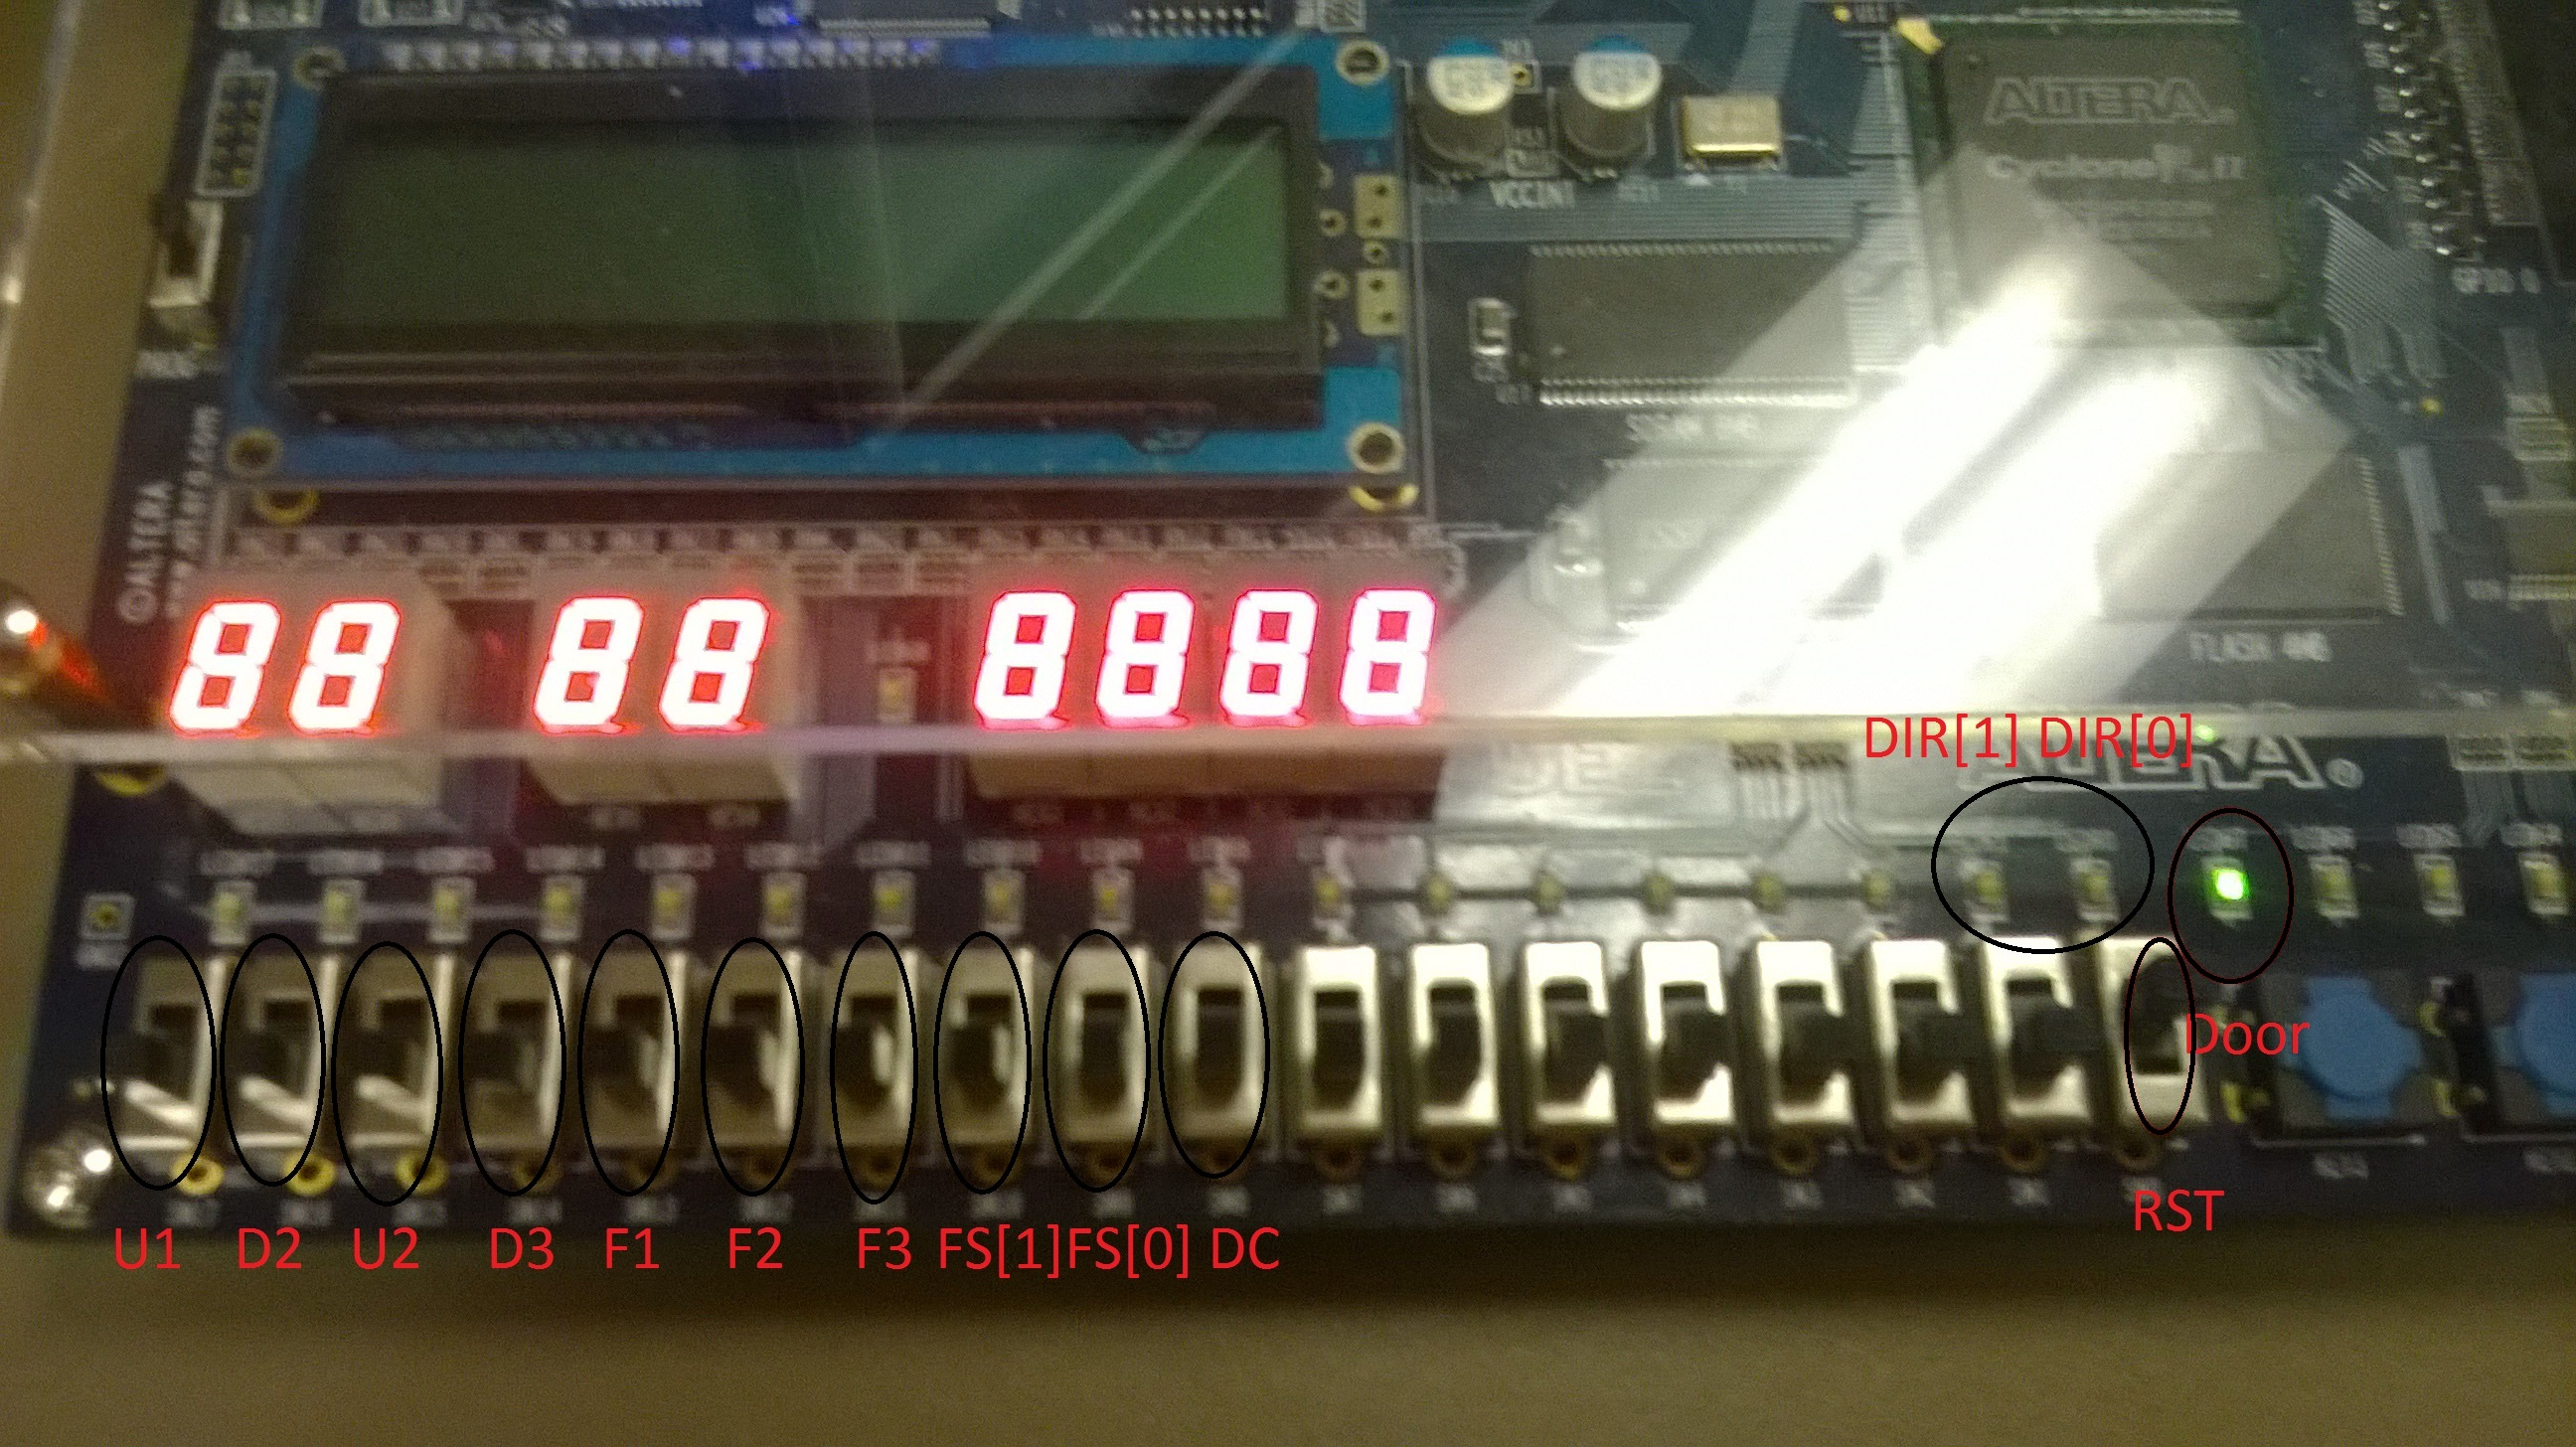
\includegraphics[width=0.9\linewidth]{Altera_Config.jpg}
\caption{Configuration of Elevator Controller on Altera board.}
\label{altera_configuration}
\end{figure}

% Synth State Machine
\begin{figure}[h]
\centering
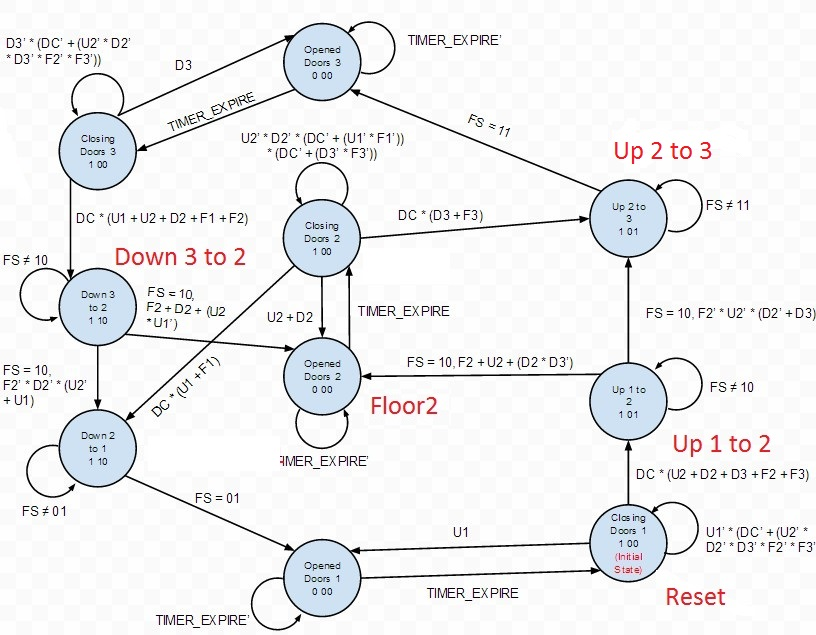
\includegraphics[width=0.9\linewidth]{Synth_State_Machine.jpg}
\caption{Add Caption.}
\label{synth_state_machine}
\end{figure}

% Reset
\begin{figure}[h]
\centering
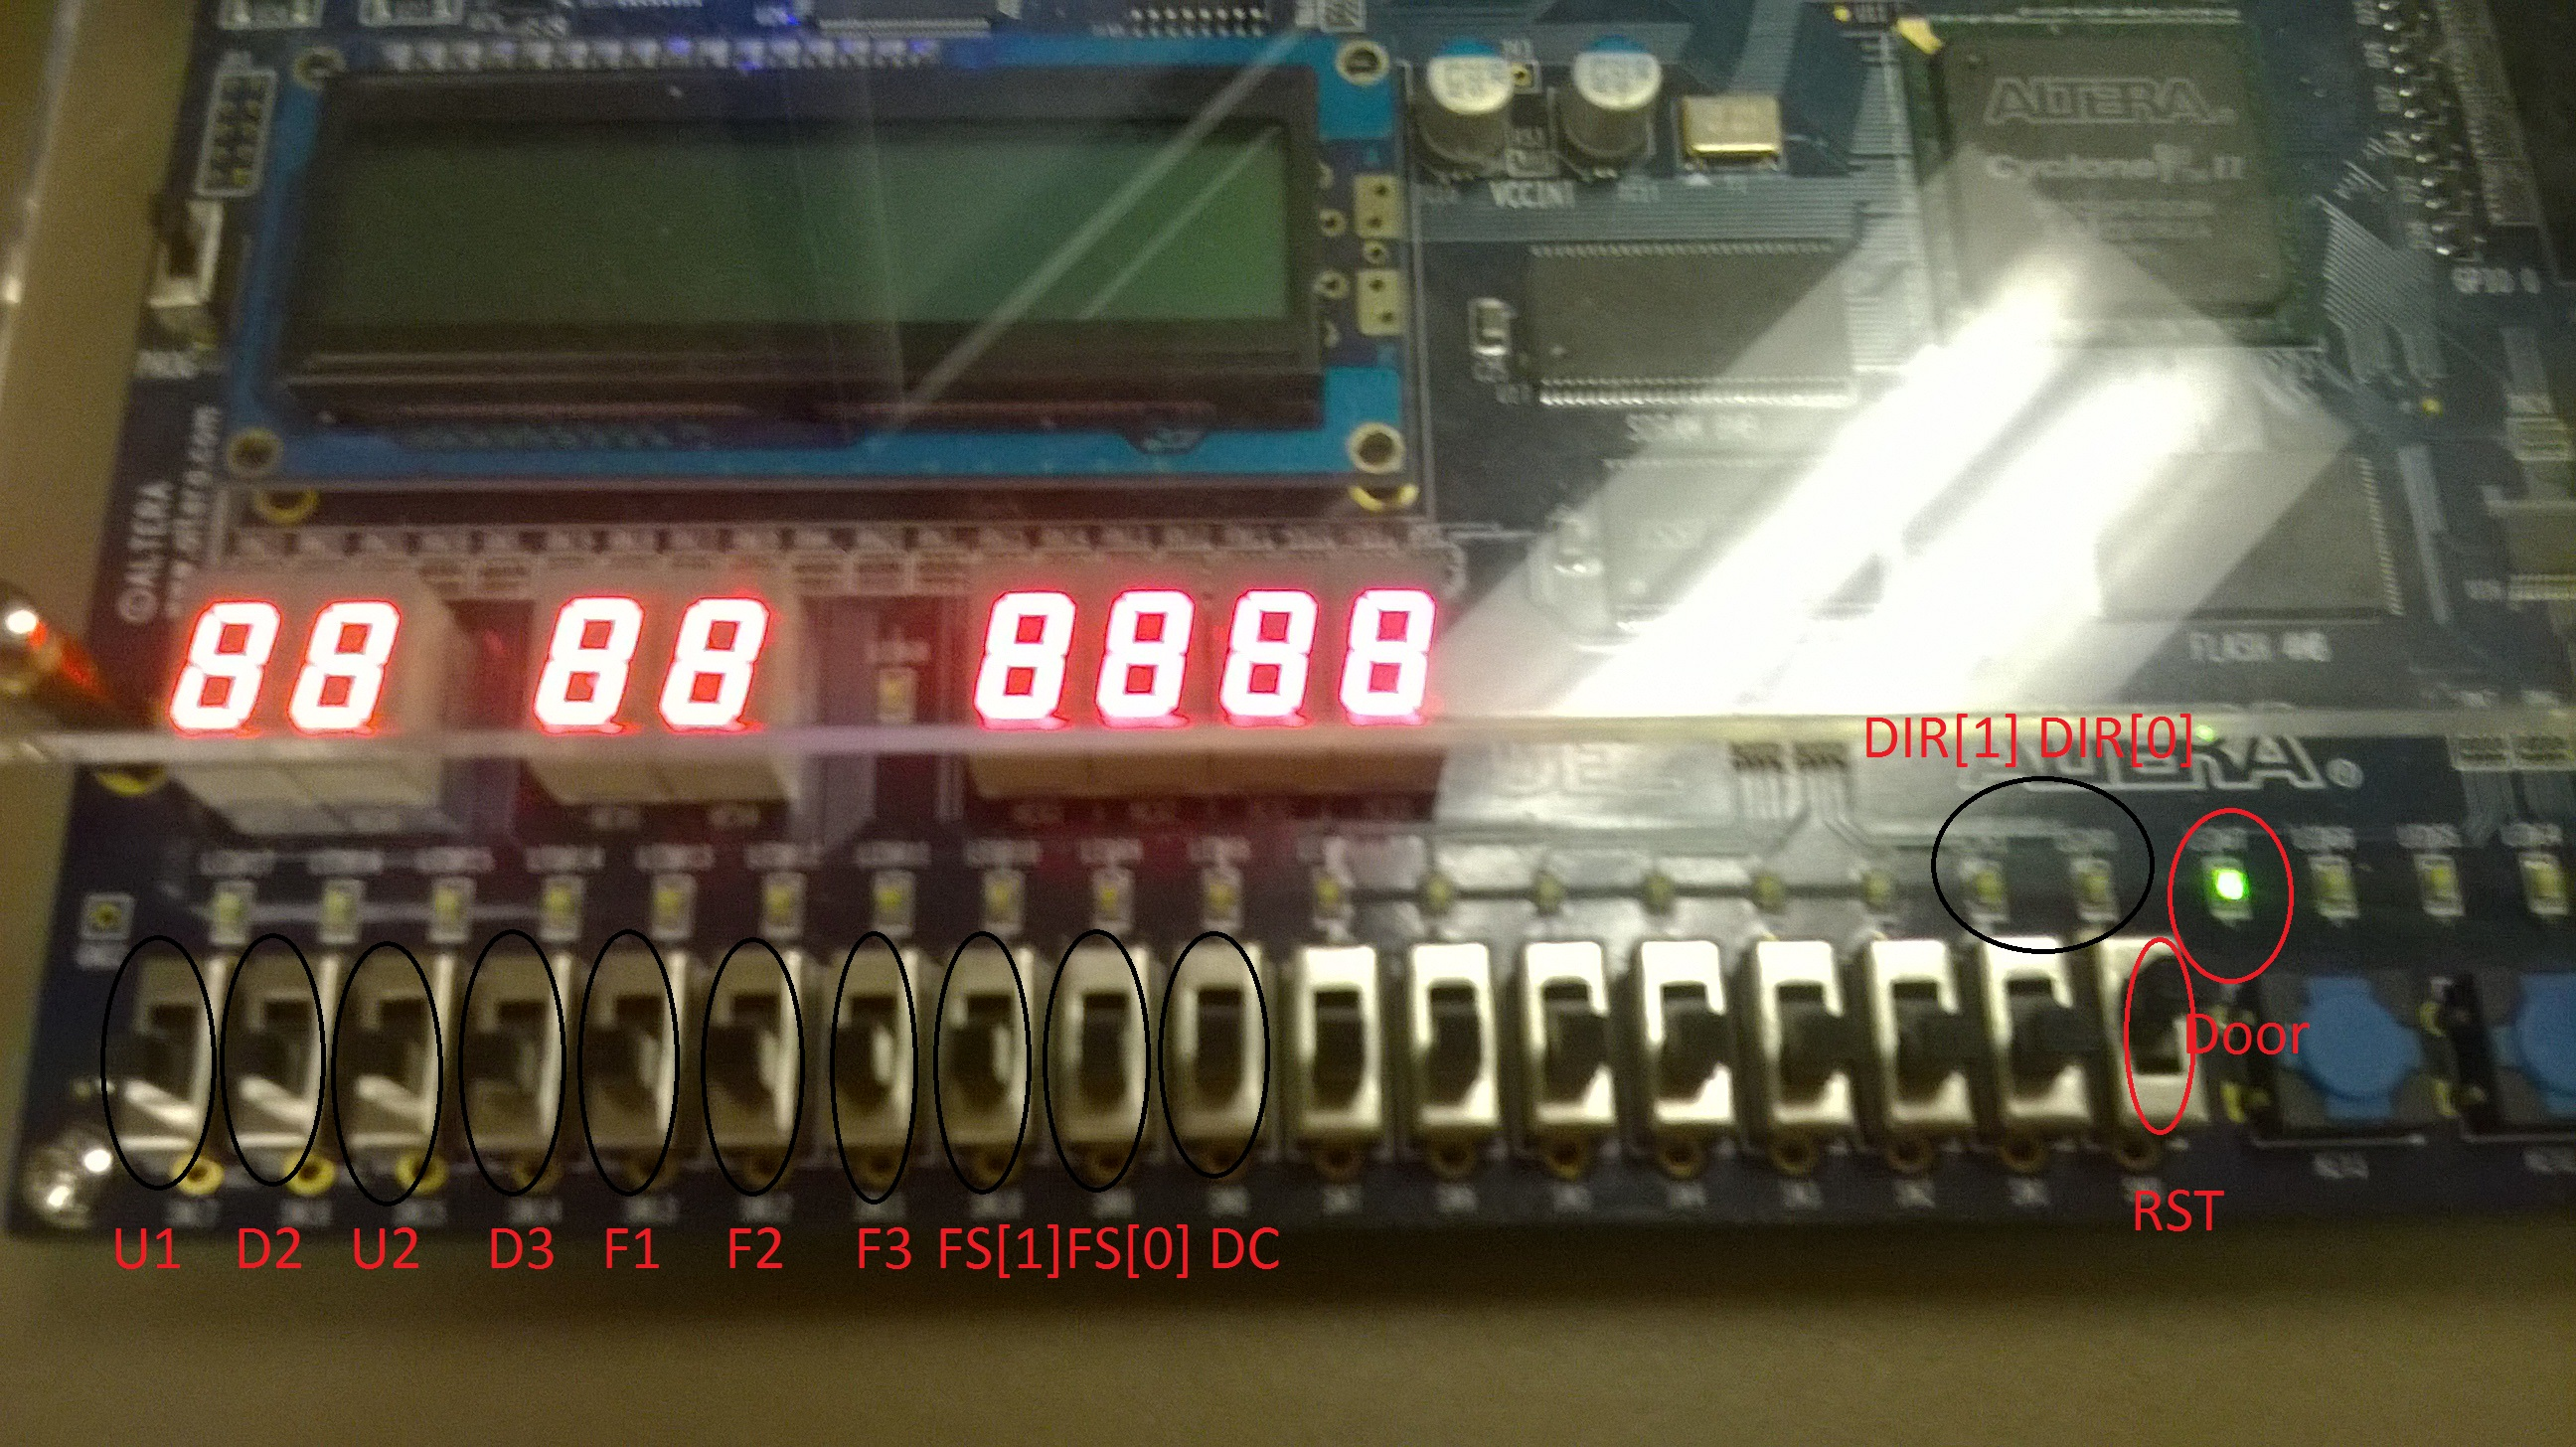
\includegraphics[width=0.9\linewidth]{Reset.jpg}
\caption{Reset.}
\label{reset}
\end{figure}

% Up1To2
\begin{figure}[h]
\centering
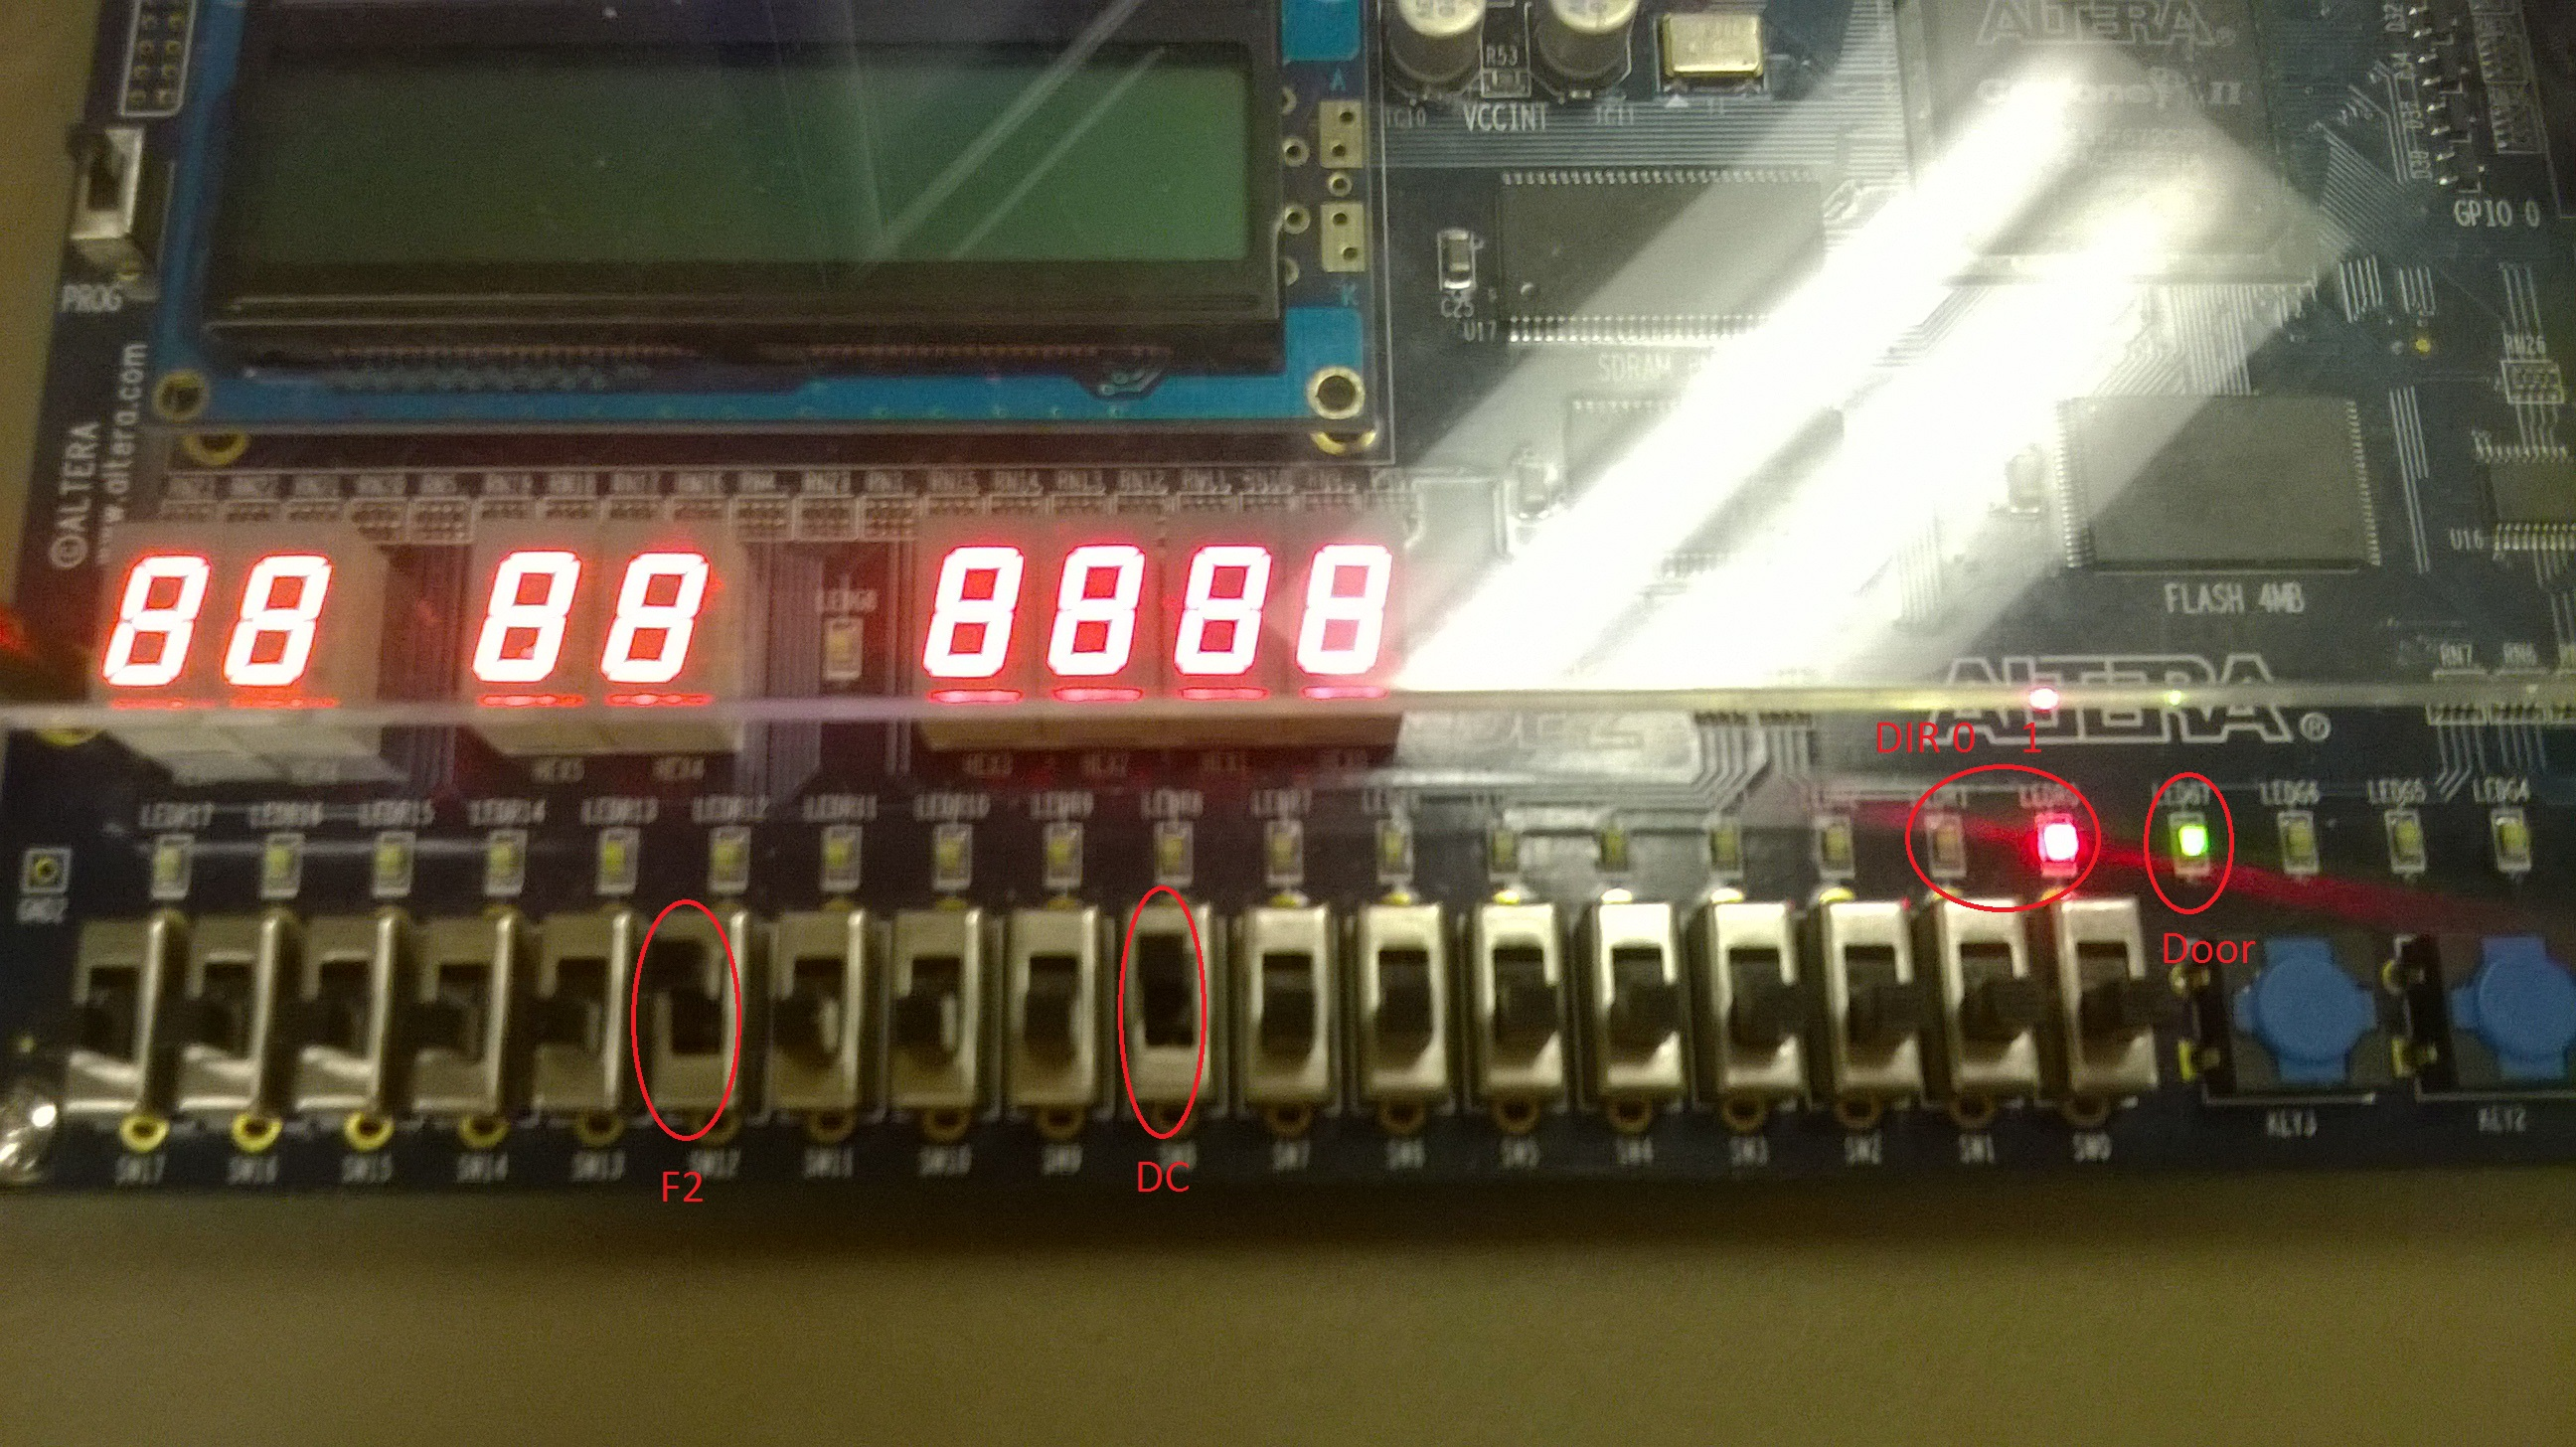
\includegraphics[width=0.9\linewidth]{Up1To2.jpg}
\caption{Up1To2 State on Altera board.}
\label{up1to2}
\end{figure}

% Floor2
\begin{figure}[h]
\centering
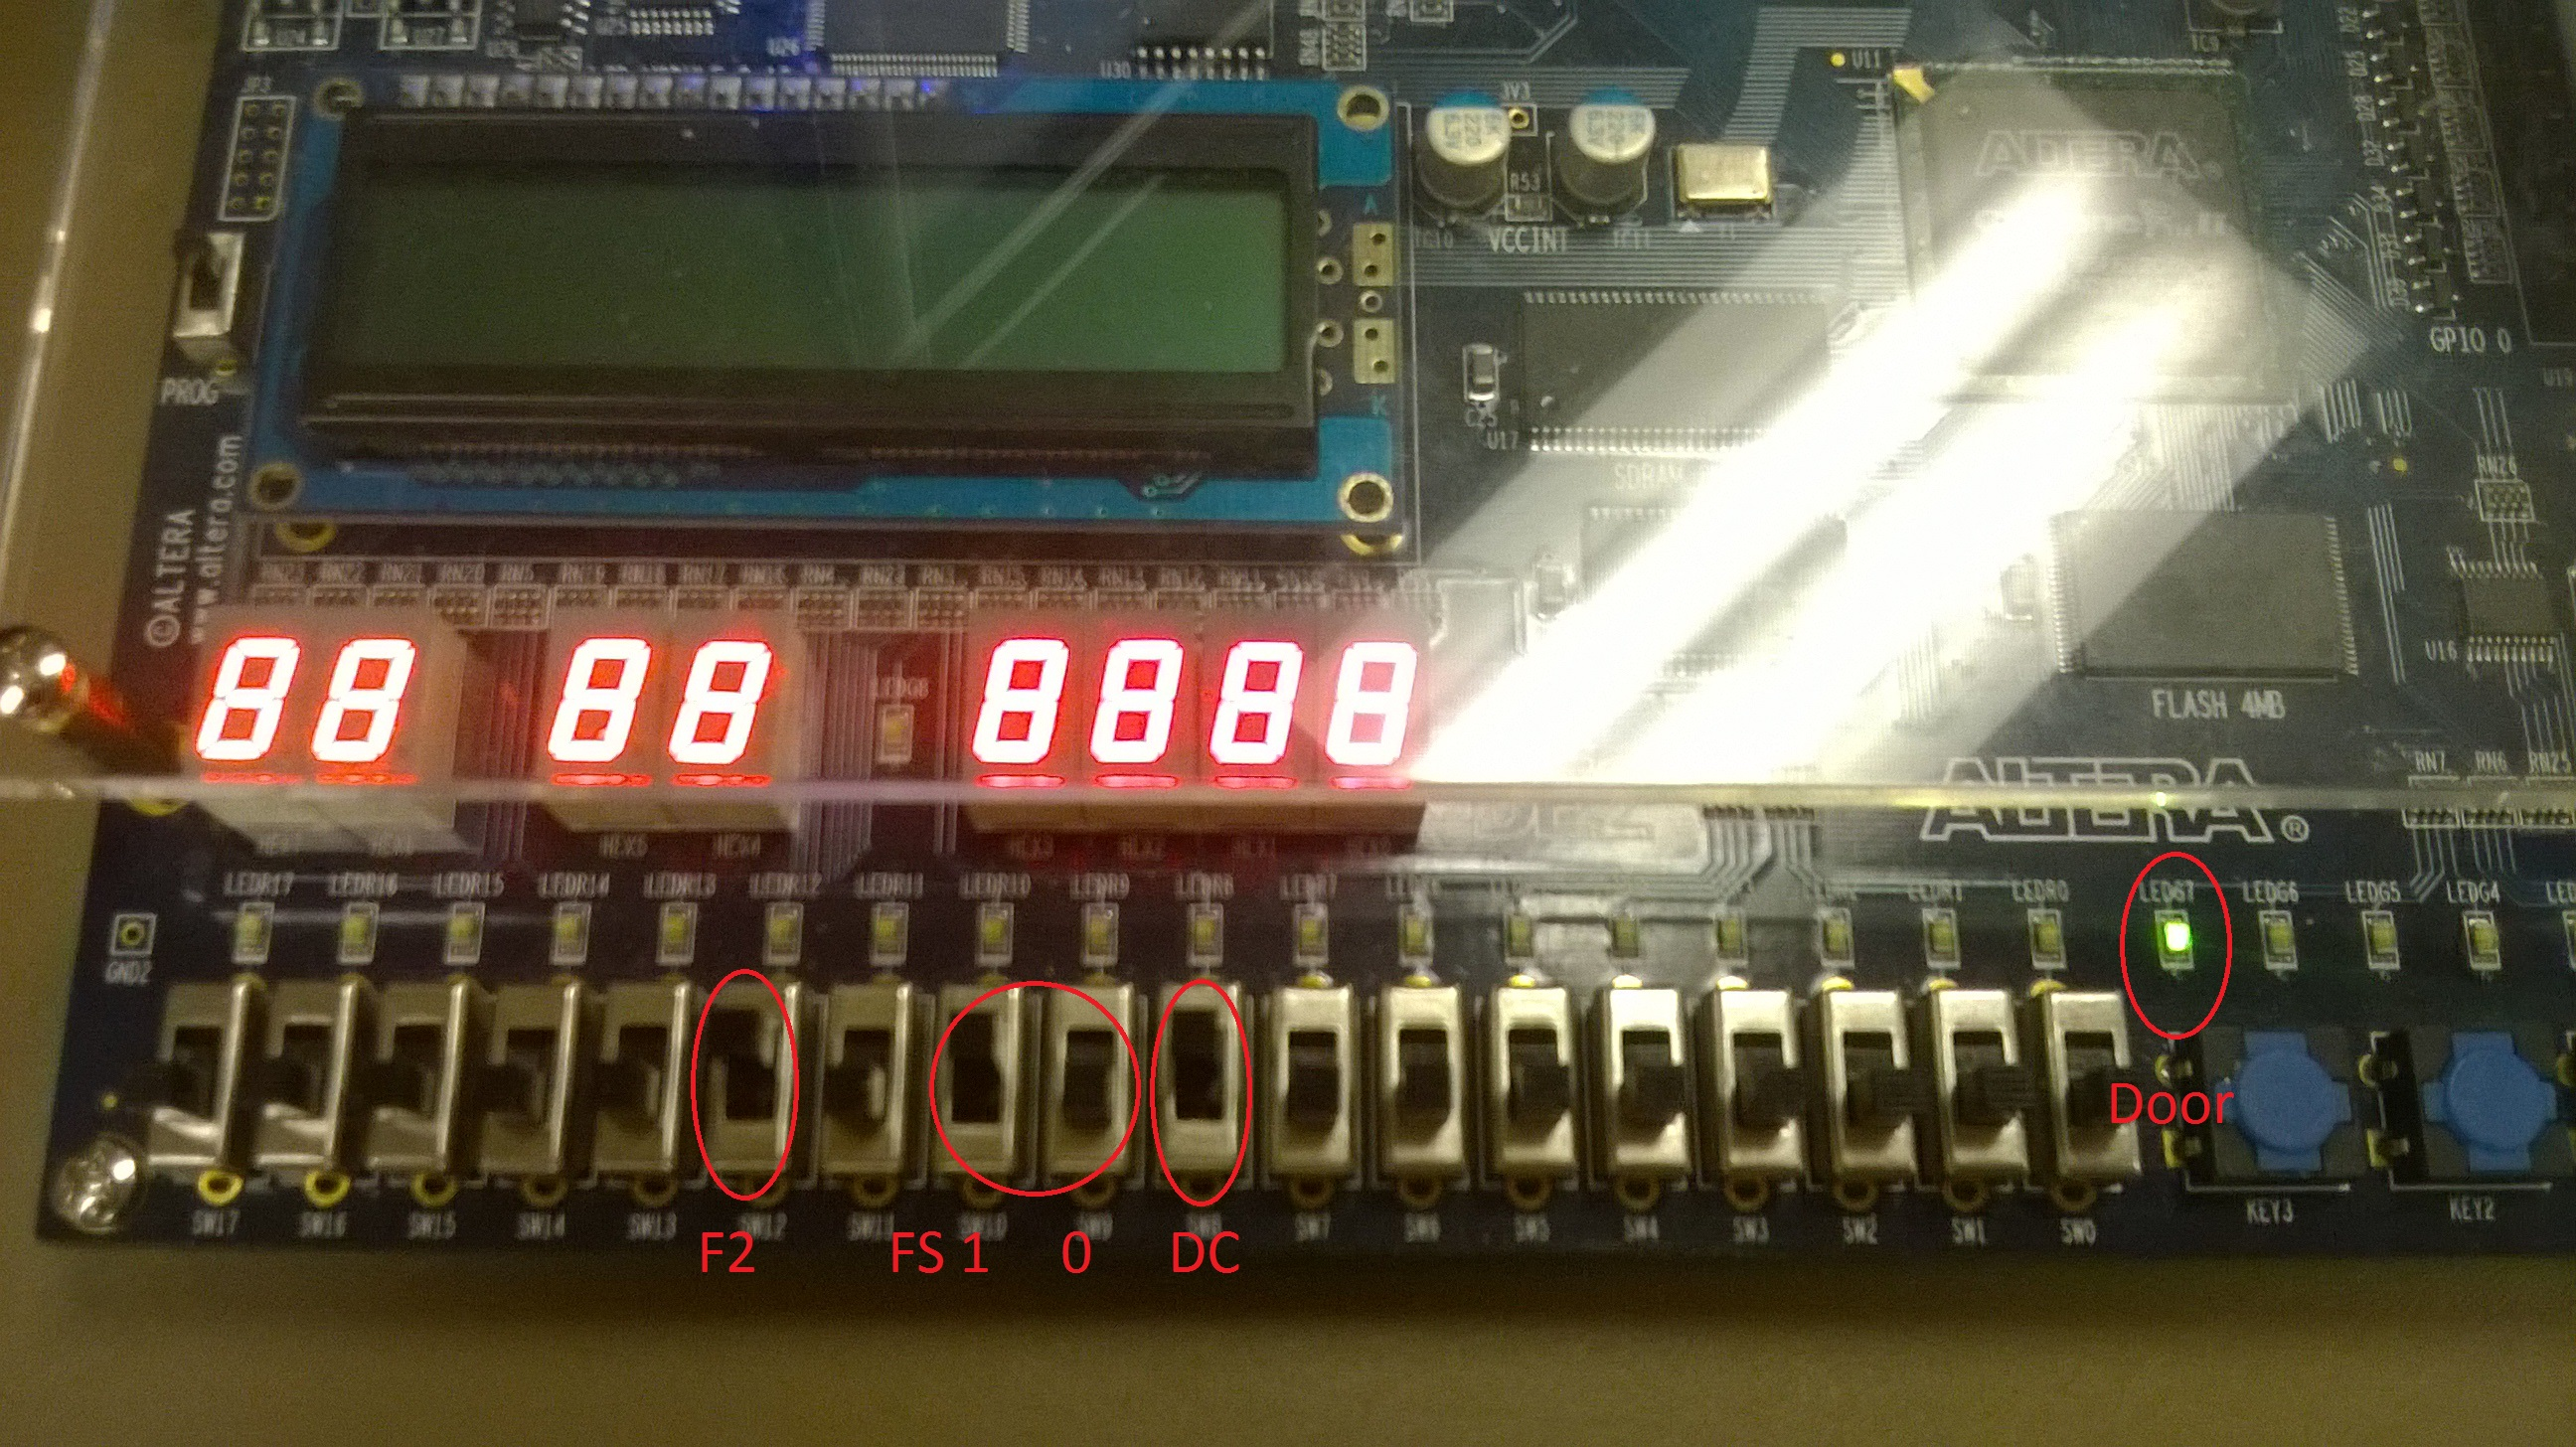
\includegraphics[width=0.9\linewidth]{Floor2.jpg}
\caption{Floor2 on Altera board.}
\label{floor2}
\end{figure}

% Up2To3
\begin{figure}[h]
\centering
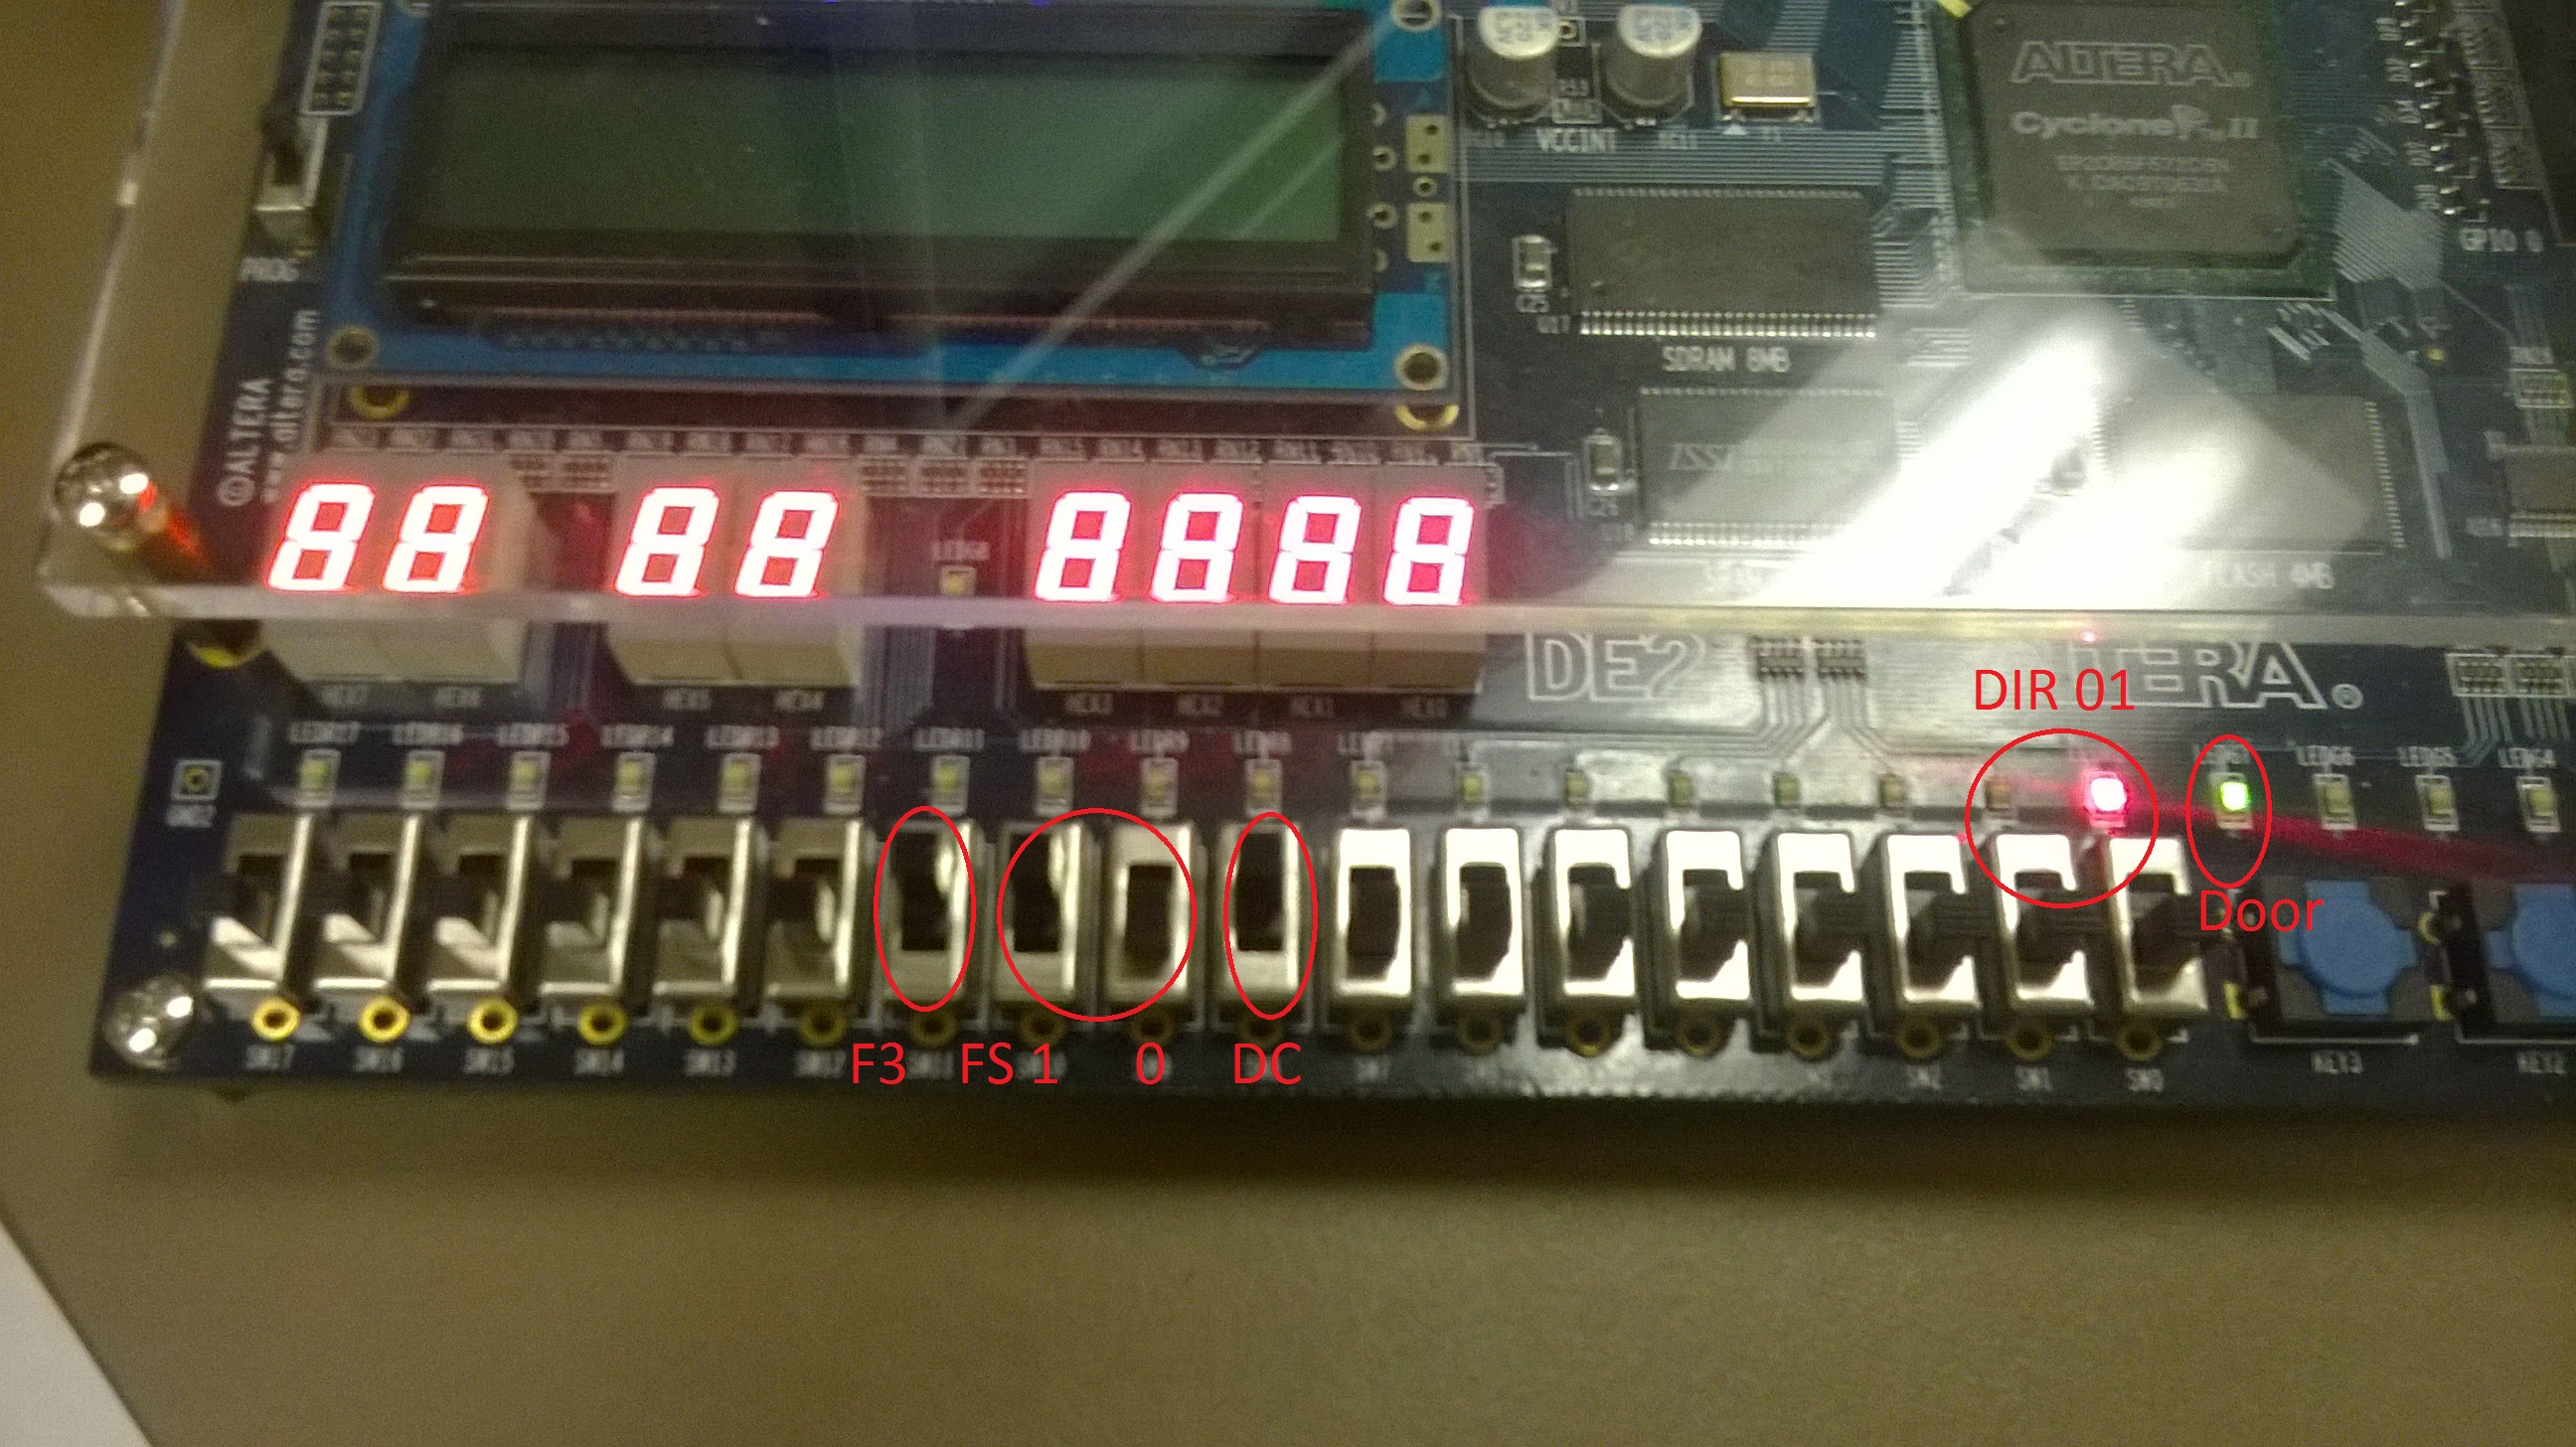
\includegraphics[width=0.9\linewidth]{Up2To3.jpg}
\caption{Up2To3 State on Altera board.}
\label{up2to3}
\end{figure}

% Down3To2
\begin{figure}[h]
\centering
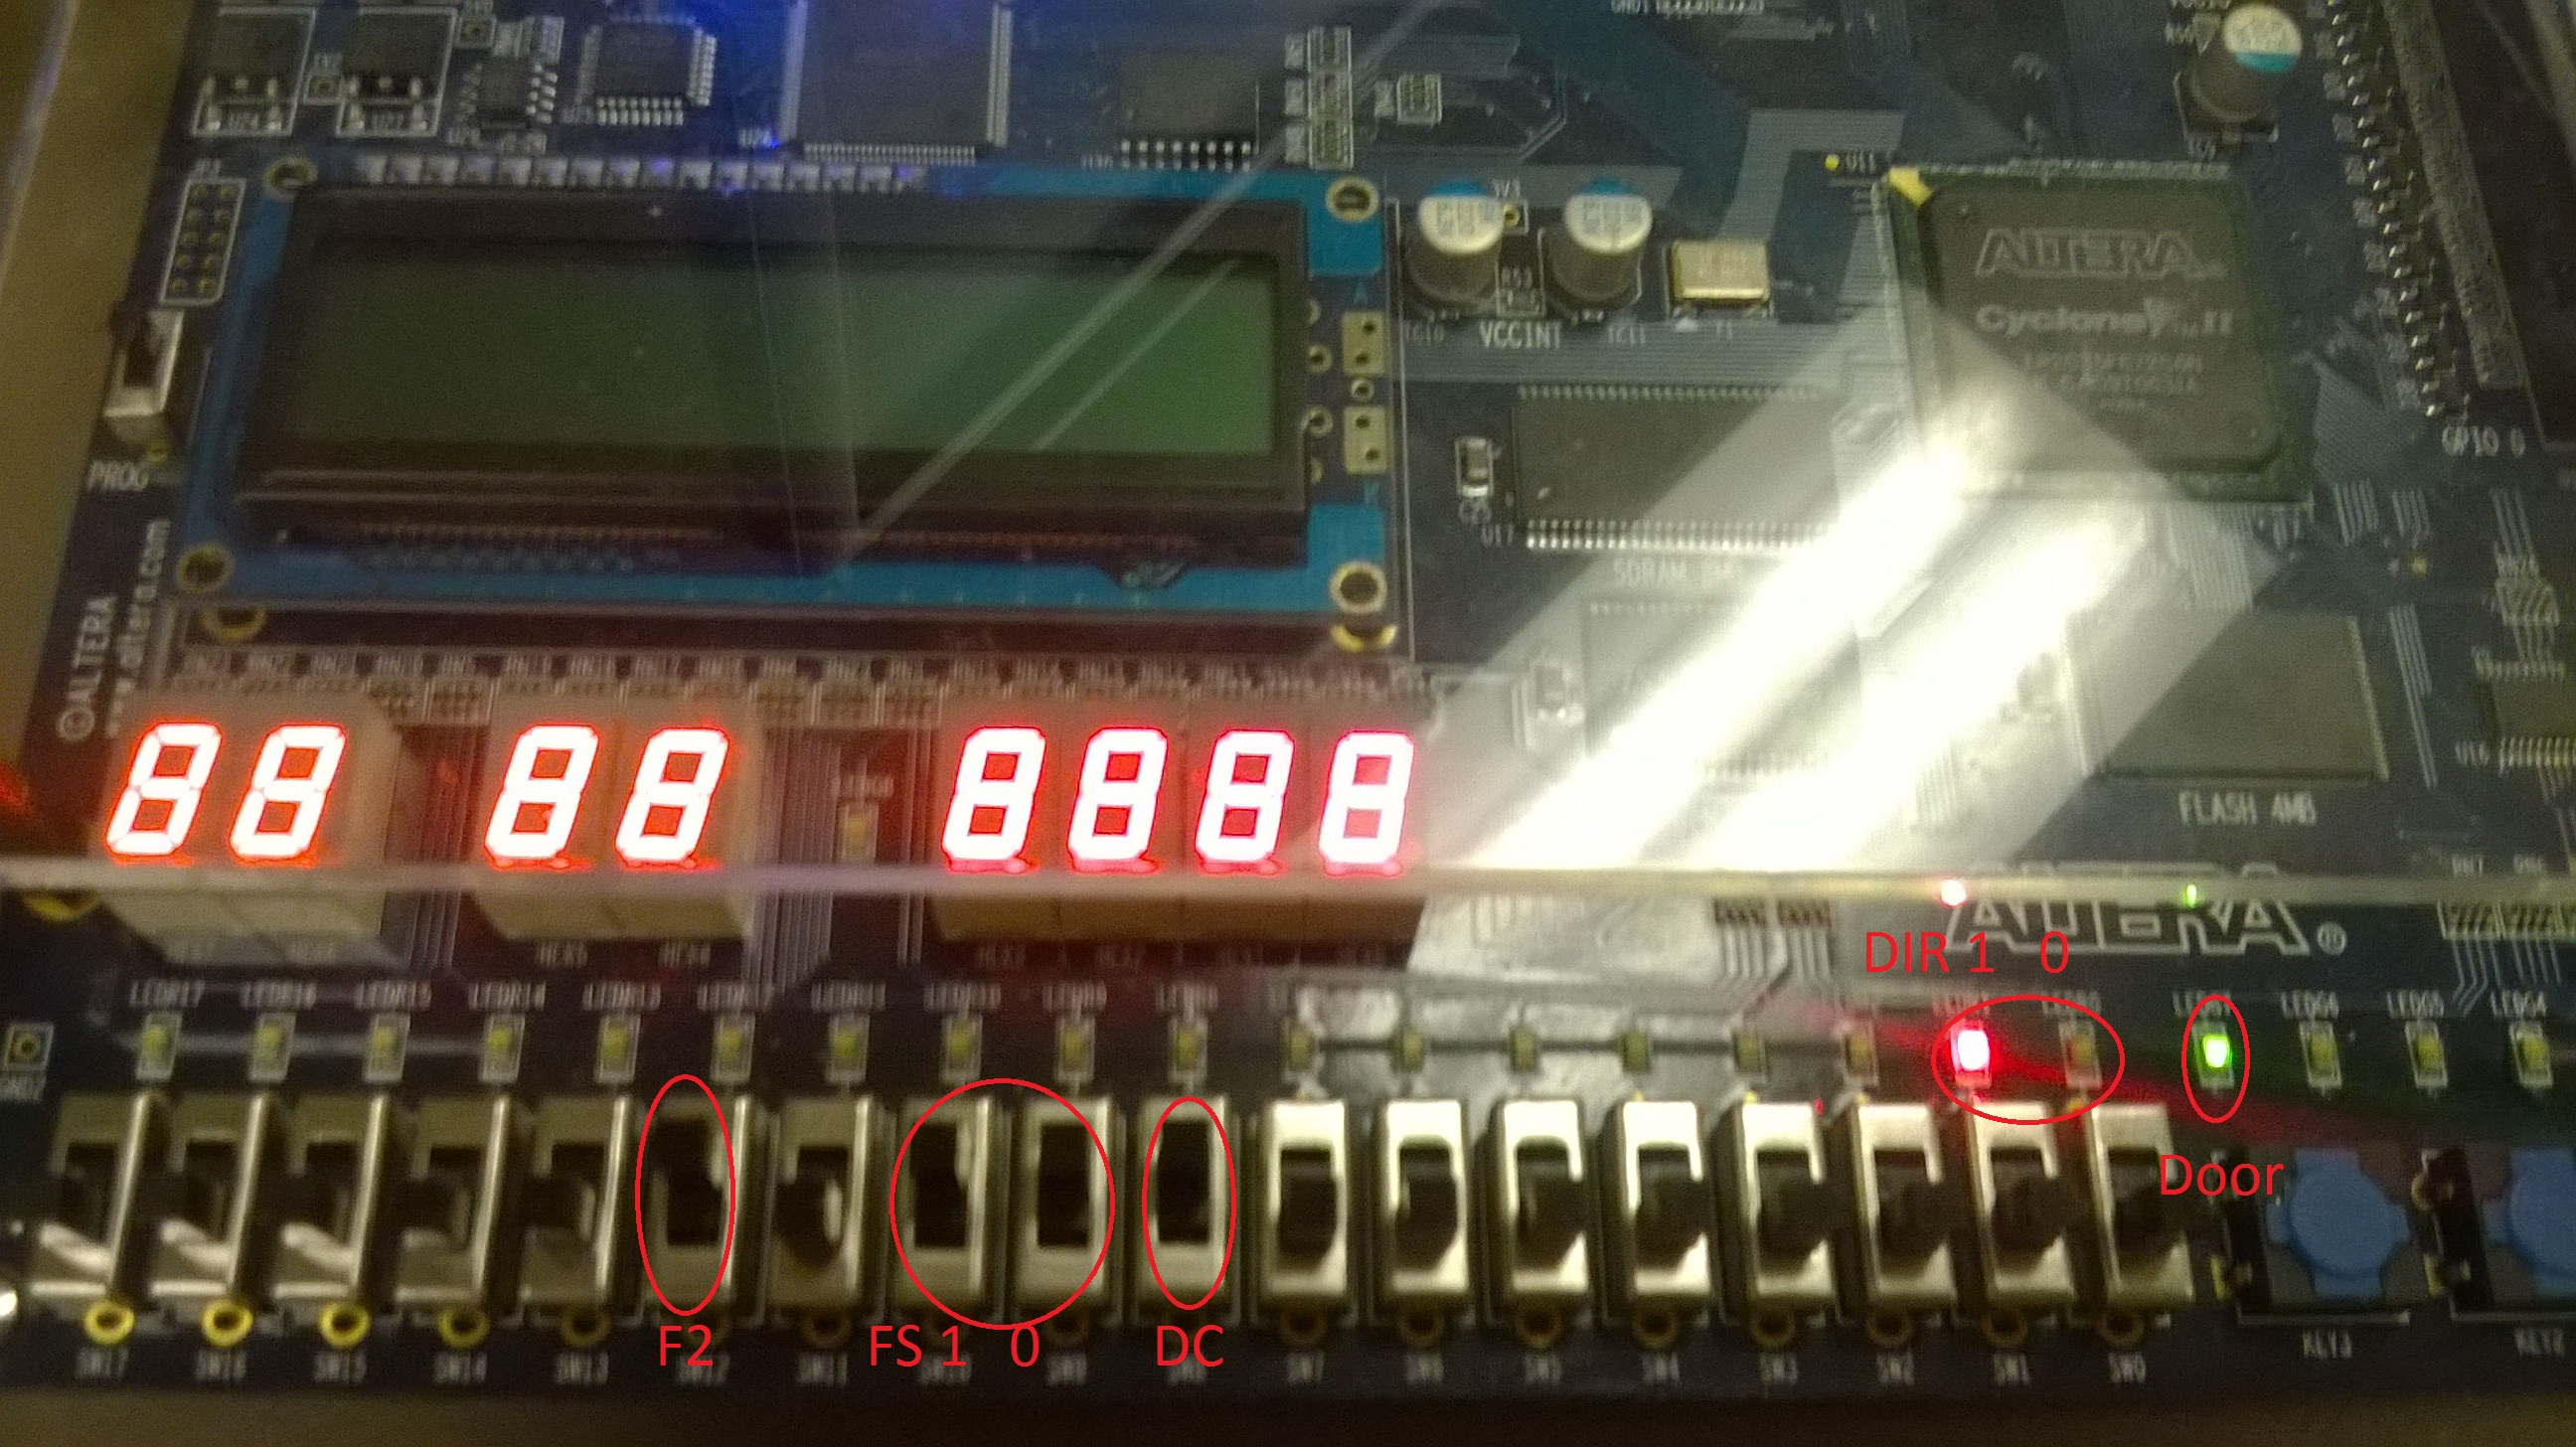
\includegraphics[width=0.9\linewidth]{Down3To2.jpg}
\caption{Down3To2 State on Altera board.}
\label{down3to2}
\end{figure}

\section{Conclusions}





% if have a single appendix:
%\appendix[Proof of the Zonklar Equations]
% or
%\appendix  % for no appendix heading
% do not use \section anymore after \appendix, only \section*
% is possibly needed

% use appendices with more than one appendix
% then use \section to start each appendix
% you must declare a \section before using any
% \subsection or using \label (\appendices by itself
% starts a section numbered zero.)
%


\appendices
\section{Model}
*Insert model here.*

% you can choose not to have a title for an appendix
% if you want by leaving the argument blank
%\section{}
%Appendix two text goes here.


% use section* for acknowledgement
\section*{Acknowledgment}


The authors would like to thank...


% Can use something like this to put references on a page
% by themselves when using endfloat and the captionsoff option.
\ifCLASSOPTIONcaptionsoff
  \newpage
\fi



% trigger a \newpage just before the given reference
% number - used to balance the columns on the last page
% adjust value as needed - may need to be readjusted if
% the document is modified later
%\IEEEtriggeratref{8}
% The "triggered" command can be changed if desired:
%\IEEEtriggercmd{\enlargethispage{-5in}}

% references section

% can use a bibliography generated by BibTeX as a .bbl file
% BibTeX documentation can be easily obtained at:
% http://www.ctan.org/tex-archive/biblio/bibtex/contrib/doc/
% The IEEEtran BibTeX style support page is at:
% http://www.michaelshell.org/tex/ieeetran/bibtex/
%\bibliographystyle{IEEEtran}
% argument is your BibTeX string definitions and bibliography database(s)
%\bibliography{IEEEabrv,../bib/paper}
%
% <OR> manually copy in the resultant .bbl file
% set second argument of \begin to the number of references
% (used to reserve space for the reference number labels box)
\begin{thebibliography}{1}

\bibitem{IEEEhowto:kopka}
H.~Kopka and P.~W. Daly, \emph{A Guide to \LaTeX}, 3rd~ed.\hskip 1em plus
  0.5em minus 0.4em\relax Harlow, England: Addison-Wesley, 1999.

\end{thebibliography}


% that's all folks
\end{document}


